\documentclass[11pt]{article}

% ===== Geometry & typography =====
\usepackage[margin=1in,letterpaper]{geometry}
\usepackage[T1]{fontenc}
\usepackage[utf8]{inputenc}
\usepackage{lmodern}
\usepackage{microtype}
\usepackage{setspace}\setstretch{1.06}

% ===== Math =====
\usepackage{amsmath,amssymb,amsfonts,amsthm,mathtools,bm}

% ===== Figures, tables, code =====
\usepackage{graphicx}
\usepackage{booktabs,array,multirow,longtable}
\usepackage{caption}\captionsetup{font=small,labelfont=bf}
\usepackage{subcaption}
\usepackage{listings}
\usepackage{enumitem}
\usepackage{float}
\usepackage{xcolor}
\definecolor{cb}{HTML}{1f77b4}
\definecolor{cr}{HTML}{d62728}
\definecolor{cg}{HTML}{2ca02c}
\definecolor{cy}{HTML}{8c6d31}
\definecolor{codebg}{RGB}{245,245,245}
\lstset{basicstyle=\ttfamily\footnotesize,frame=single,framerule=0.3pt,
  rulecolor=\color{gray!50},backgroundcolor=\color{codebg},
  keywordstyle=\color{cb}\bfseries,commentstyle=\color{gray!60},language=Python,
  showstringspaces=false,numbersep=4pt,xleftmargin=8pt,xrightmargin=4pt,
  breaklines=true}

% ===== TikZ =====
\usepackage{tikz}
\usetikzlibrary{arrows.meta,positioning,calc,fit,shapes.geometric,backgrounds,
  decorations.pathreplacing,decorations.pathmorphing,decorations.markings,matrix,patterns,automata}

% ===== References & hyperlinks =====
\usepackage[hidelinks]{hyperref}
\usepackage{cleveref}\crefname{equation}{Eq.}{Eqs.}\crefname{section}{\S}{\S\S}

% ===== Theorem-like environments =====
\newtheoremstyle{plain1}{8pt}{8pt}{\itshape}{}{\bfseries}{.}{0.6em}{}
\newtheoremstyle{definition1}{8pt}{8pt}{}{}{\bfseries}{.}{0.6em}{}
\theoremstyle{plain1}
\newtheorem{theorem}{Theorem}
\newtheorem{proposition}[theorem]{Proposition}
\newtheorem{lemma}[theorem]{Lemma}
\theoremstyle{definition1}
\newtheorem{definition}{Definition}
\newtheorem*{remark}{Remark}
\newtheorem*{takeaway}{Takeaway}

% ===== Math shorthands =====
\newcommand{\R}{\mathbb{R}}
\newcommand{\E}{\mathbb{E}}
\newcommand{\Prb}{\mathbb{P}}
\newcommand{\Var}{\mathrm{Var}}
\newcommand{\Cov}{\mathrm{Cov}}
\newcommand{\argmax}{\operatorname*{arg\,max}}
\newcommand{\argmin}{\operatorname*{arg\,min}}
\newcommand{\1}{\mathbf{1}}
\newcommand{\bel}{\mathbf{b}}
\newcommand{\state}{\mathcal{S}}
\newcommand{\action}{\mathcal{A}}
\newcommand{\Obs}{\mathcal{O}}

% ===== Title block =====
\title{
  \Large \textbf{Regime-Switching Asset Allocation via a POMDP:\\
   A Methods Stress-Test with Twelve Baselines and Three Diagnostic Regressions} \\[3pt]
  \normalsize \textit{Extended Technical Report}
}
\author{
  Dario Blanco Morales \quad Even Hogberget \quad Kyle David Ledda-Lewaren \quad Taka Khoo \\[2pt]
  \small ENGS 177: Decision Making Under Uncertainty, Spring 2026 \\
  \small Thayer School of Engineering, Dartmouth College
}
\date{May 2026}

\begin{document}
\maketitle

%================================================
\begin{abstract}\noindent
We model dynamic stock-bond allocation as a Partially Observable Markov Decision Process (POMDP) whose latent state is the prevailing macro-financial regime, infer regimes from a Gaussian Hidden Markov Model (HMM) fit by Baum--Welch, and act with the QMDP approximation. The headline question is whether a decision-theoretic regime overlay beats a static $60/40$ benchmark out-of-sample over $2003$--$2026$ on SPY and AGG.

This extended report extends the original 10-page deliverable in five directions:
(1)~we add eight macro-financial observation channels (T10Y2Y, NFCI, STLFSI4, UMCSENT, ICSA, USD index, WTI oil, Fed funds);
(2)~we implement eleven new baseline strategies, including risk parity (Maillard--Roncalli--Teiletche), Markowitz with Ledoit--Wolf shrinkage, Faber 10-month moving average, time-series momentum, vol-targeting, HMM-conditional mean-variance (Guidolin--Timmermann), and Black--Litterman with HMM-derived views;
(3)~we re-frame the project using Powell's (2019) four-class taxonomy of policies for sequential decision-making (PFA / CFA / VFA / DLA), positioning QMDP explicitly as a VFA combined with a one-step DLA;
(4)~we run two diagnostic experiments: a feature-cohort study testing whether richer observations break the QMDP collapse, and a walk-forward refit study testing whether the Nystrup--Madsen--Lindstr\"om (2018) protocol changes the headline verdict; and
(5)~we situate every theoretical claim against published results (Singh \& Sutton 1996, Singh et al.\ 2000, Watkins \& Dayan 1992, Van Hasselt 2010, Precup et al.\ 2000, Jaakkola et al.\ 1994, Auer et al.\ 2002, Hauskrecht 2000, Pineau et al.\ 2003, Hamilton 1989, Ang \& Bekaert 2002, Guidolin \& Timmermann 2007, Nystrup et al.\ 2018, Tu 2010).

The substantive findings are three-fold. First, in the original configuration (two observation channels, fixed in-sample HMM, CRRA $\gamma{=}2$), QMDP collapses to ``100\% stocks'' in both regimes and underperforms 60/40 on Sharpe (0.73 vs.\ 0.81). The empirical winner of a twelve-strategy horse race is the Faber 10-month-SMA rule (Sharpe 1.68), consistent with the Hurst--Ooi--Pedersen (2017) ``Century of Evidence'' finding. Second, adding the Chicago Fed NFCI and St.\ Louis Fed STLFSI4 as observation channels breaks the policy collapse: the optimal MDP policy becomes regime-dependent (100/0 in bull, 0/100 in bear) at the same $\gamma{=}2$. Third, switching from a fixed in-sample HMM to an expanding-window walk-forward refit lifts QMDP Sharpe from 0.81 to 1.08 and cuts max drawdown from $-34\%$ to $-16\%$. The original ``QMDP loses'' headline therefore holds only in the specific joint configuration of (a) narrow VIX$+$spread observations, (b) fixed HMM, (c) low CRRA. Each component is empirically reversible, consistent with Tu's (2010) framing that regime-switching benefits depend strongly on parameterisation. We close with three methodological extensions (point-based VI; off-policy evaluation via importance sampling; CVaR-penalised reward) and an honest verdict: the practitioner consensus winner for two-asset tactical allocation (trend $+$ vol-target $+$ cash fallback) remains best, but QMDP can be made competitive with proper methodology.
\end{abstract}

\bigskip\hrule\medskip
\tableofcontents
\bigskip\hrule

%================================================
\section{Introduction}\label{sec:intro}
%================================================

\subsection{The empirical problem}

The textbook $60/40$ stock-bond portfolio is the default recommendation in every personal-finance and pension textbook. It assumes returns are approximately stationary: stocks pay a risk premium, bonds diversify, and the mix is set-and-forget. Reality violates this assumption in two specific ways. First, returns are \emph{conditionally heteroskedastic}: long quiet periods are interrupted by short, sharp crises (2008, 2020, 2022). Second, stress periods exhibit \emph{higher cross-asset correlations}: stocks and bonds sell off together precisely when the diversification benefit is most needed. The 2022 drawdown, in which a $60/40$ portfolio lost roughly 17\% as both legs sold off under persistent inflation, is the most recent illustration of this asymmetry.

\subsection{The research question}

Whether to \emph{think} about regimes is not new. The literature is decades old: Hamilton (1989) introduced the two-state Markov-switching model for U.S.\ GDP; Ang and Bekaert (2002) demonstrated welfare losses from ignoring regimes in international asset allocation; Guidolin and Timmermann (2007) formalised multi-asset allocation under regime switching as a dynamic-programming problem; Nystrup et al.\ (2018) addressed walk-forward refit. What is less settled is the following \emph{methodological} question:
\begin{center}\itshape
Can a fully decision-theoretic regime overlay---formalised as a POMDP, fit to public macro-financial data, solved by a tractable belief-state heuristic---beat the static $60/40$ benchmark out-of-sample after realistic transaction costs?
\end{center}

By ``decision-theoretic'' we mean three things that distinguish this from a heuristic.
\begin{enumerate}[leftmargin=2em]
  \item The allocation rule is the \emph{solution of an explicit optimisation}, not a discretionary rule of thumb.
  \item The latent regime is treated as a \emph{hidden state} and inferred by a \emph{Bayesian filter}, not labelled by hand.
  \item The policy is the \emph{QMDP approximation of an underlying POMDP}, which makes it \emph{falsifiable, comparable, and explainable}.
\end{enumerate}
The hypothesis we stress-test is the \emph{implicit claim} of every regime-switching paper: that the static $60/40$ leaves Sharpe ratio on the table because it ignores the regime label.

\subsection{Why POMDP, not a tree, not an MDP}

Three observations together force the POMDP formulation, each ruling out a simpler model.
\begin{enumerate}[leftmargin=2em]
  \item Decision tree: the tree explodes combinatorially with horizon; no shared state representation.
  \item Influence diagram: same blow-up; not natural for a repeated monthly rebalance.
  \item Fully observable MDP: requires us to \emph{know} the current regime. We do not---it is latent.
  \item POMDP (ours): hidden state, noisy observations, sequential decisions, belief updates. Exactly our setting.
\end{enumerate}

\subsection{What would falsify the methodology}

A clean win for the methodology requires three conditions:
QMDP Sharpe $>$ static $60/40$ Sharpe; the optimal policy \emph{differs across regimes} (bull vs.\ bear); and the improvement survives transaction costs. A clean loss requires QMDP Sharpe $\leq$ static or a regime-insensitive policy. Our headline finding, in the original two-channel fixed-HMM configuration, is closer to a loss than a win.

\subsection{Contributions of this extended report}

We make seven specific contributions over the original 10-page report.
\begin{enumerate}[leftmargin=2em,itemsep=2pt]
  \item \textbf{Eight additional observation channels} fetched from FRED (\Cref{sec:data}).
  \item \textbf{Eleven additional baseline strategies} (\Cref{sec:baselines}) spanning the academic and practitioner consensus.
  \item \textbf{Twelve-strategy horse-race backtest} on the identical 2003--2026 universe (\Cref{sec:horserace}).
  \item \textbf{Multi-feature HMM cohort study} testing whether richer observations break the QMDP policy collapse (\Cref{sec:feature-cohort}).
  \item \textbf{Walk-forward refit study} testing whether the Nystrup et al.\ (2018) protocol changes the headline verdict (\Cref{sec:walk-forward}).
  \item \textbf{Theoretical repositioning} via Powell's (2019) four-class taxonomy and explicit grounding in the supplementary papers (\Cref{sec:powell}).
  \item \textbf{Public reproducible repository} \texttt{takakhoo/ENGS177\_Final\_Project} containing all data (745~KB), 12 Python modules, and 10 experiment scripts.
\end{enumerate}

%================================================
\section{Background and Related Work}\label{sec:related}
%================================================

\subsection{Regime switching in finance}

The two-state Markov-switching model originates with \textbf{Hamilton (1989)} for U.S.\ GDP. \textbf{Ang \& Bekaert (2002)} extended the framework to international equity allocation: their headline result is that ``costs of ignoring regimes are small for all-equity portfolios but become economically meaningful only when the investor can hold a conditionally risk-free asset.'' This is directly relevant to our negative finding: in our two-risky-asset SPY/AGG universe, there is no risk-free leg to switch into, so the regime label's marginal value is small.

\textbf{Guidolin \& Timmermann (2007)} formalise multi-asset regime-switching allocation as a CRRA dynamic-programming problem with a \emph{four-state} HMM (crash, slow growth, bull, recovery). Their qualitative result: optimal allocations to stocks vary considerably across states; certainty-equivalent annual gain over static is on the order of 1--2\%. Their methodological message is that \emph{2-state HMMs with risky-only universes typically fail to produce regime-dependent policies}---exactly the scenario in our original headline configuration.

\textbf{Tu (2010)} explicitly examines whether regime switching matters once model, parameter, and regime uncertainty are jointly accounted for in a Bayesian framework. His answer is qualified: certainty-equivalent loss from ignoring regimes is generally 2\%/year and up to 10\% at high risk aversion---but the binding mechanism is the cash-switching trick, not the regime label changing the equity-vs-bond mix in a CRRA-without-cash setup. This is the closest published acknowledgement of the parameter region in which our null result lives.

\textbf{Nystrup, Madsen, Lindstr\"om (2018, \emph{Quantitative Finance} 18(1))} introduce the canonical walk-forward HMM-refit protocol: a 2-state HMM with online (recursive) re-estimation, applied to monthly multi-asset returns, with the regime signal subject to a 1-day delay. The strategy outperforms a static benchmark in Sharpe and especially in max drawdown, but only when regime persistence exceeds the inference latency. Our \Cref{sec:walk-forward} re-runs our QMDP under this protocol and reproduces their qualitative finding.

\textbf{Bulla et al.\ (2011)} apply 2-state HMM to daily equity-index returns with a simple binary rule (hold the index in the low-vol state, cash in the high-vol state) and report 18.5--201.6 bp/year excess returns---but the strategy is fundamentally a \emph{vol-timing / cash-switching} rule, not an alpha-generation rule. Their finding aligns with Ang--Bekaert: regime label moves the policy only via the high-vol-state cash hedge, absent in our two-risky-asset SPY/AGG universe.

\textbf{Kritzman, Page \& Turkington (2012)} use 2-state Markov switching on \emph{market turbulence, inflation, and economic growth}---macro/financial state variables rather than returns themselves. Their feature choice is close in spirit to ours (VIX and term spread).

\subsection{POMDP / QMDP in finance}

\textbf{Hauskrecht (2000, \emph{JAIR} 13)} is the reference for QMDP, the Fast Informed Bound (FIB), and the family of upper-bound approximations. Crucially for our framing, Hauskrecht shows QMDP cannot motivate information-gathering actions. Since in our setup there is \emph{no action that improves observability of the regime}---we observe (VIX, term spread) regardless of allocation---QMDP is asymptotically near-optimal in our problem class. \textbf{Littman, Cassandra \& Kaelbling (1995)} is the original QMDP paper. \textbf{Pineau, Gordon \& Thrun (2003)} introduce point-based value iteration (PBVI) as the canonical tighter alternative; on our 2-latent-state $K{=}2$ problem with a 1-dimensional belief simplex, PBVI is unnecessary.

POMDP framings of portfolio choice are otherwise \emph{rare} in the finance literature: continuous-time relatives exist (Dai, Zhang, Zhu 2010; Sass \& Haussmann 2004) but they use HJB methods rather than discrete POMDP / QMDP machinery. The discrete-time POMDP $+$ QMDP framing we use is genuinely uncommon---a methodological selling point.

\subsection{Powell (2019)'s unifying taxonomy}\label{sec:powell}

\textbf{Powell (2019, \emph{EJOR} 275(3))} proposes a single notational and conceptual umbrella for the fifteen overlapping communities of sequential decision-making. The universal model is
\[
\max_\pi\ \E\!\left[\, \sum_{t=0}^{T} C_t(S_t, X^\pi_t(S_t), W_{t+1}) \,\Big|\, S_0 \,\right]
\]
with state transition $S_{t+1} = S^M(S_t, x_t, W_{t+1})$ and exogenous information process $(W_1, \ldots, W_T)$. The goal is to find the best \emph{policy}, not the best decision. Powell's four meta-classes of policies are:
\begin{description}[itemsep=4pt,topsep=4pt]
  \item[Policy Function Approximations (PFAs).] Direct parametric mappings $X^\pi(S \mid \theta)$: linear features, neural networks, order-up-to rules.
  \item[Cost Function Approximations (CFAs).] $X^\pi(S \mid \theta) = \argmax_x \bar{C}^\pi(S, x \mid \theta)$ where $\bar{C}$ is a parametrically modified cost function or constraint set. \emph{UCB is a CFA} (sample mean $+$ exploration bonus).
  \item[Value Function Approximations (VFAs).] $X^\pi(S) = \argmax_x [C(S,x) + \E[\bar{V}_{t+1}(S_{t+1}) \mid S]]$. Classical ADP / RL.
  \item[Direct Lookahead Approximations (DLAs).] Solve a simplified lookahead model in real time at each state: deterministic, rollout, MCTS, two-stage stochastic programs.
\end{description}
For POMDPs (Powell \S 2.15), Powell observes that a POMDP can be reformulated as a ``belief MDP'' whose state is the belief vector $\bel^n$. Belief MDPs are notoriously hard, motivating point-based solvers and approximations.

\paragraph{Our positioning in Powell's taxonomy.}
QMDP fits naturally as a \textbf{VFA} in which the belief-state value function $V(\bel)$ is approximated by the linear lower envelope
\[
V_{\rm QMDP}(\bel) = \max_a \sum_s b(s)\, Q^\ast_{\rm MDP}(s, a),
\]
combined with a \textbf{one-step DLA} at decision time. In Powell's language we are \emph{using the MDP value function as a VFA on the belief MDP and selecting actions via a one-step direct lookahead}. This framing motivates the natural alternative design choices we discuss in \Cref{sec:conclusions}: PFAs (parameterise a direct belief $\to$ action mapping), CFAs (add an exploration bonus to the QMDP rule), full DLAs (online belief-space search like POMCP). All four classes are legitimate; we argue VFA$+$DLA is the right entry point for an undergraduate term project because it is computationally cheap, leverages an existing MDP solver, and produces an interpretable policy.

\subsection{Tactical-allocation baselines: the practitioner consensus}

The practitioner consensus across published horse races (Faber 2007/2013; Hurst--Ooi--Pedersen 2017; Asness--Frazzini--Pedersen 2012; Harvey--Liu--Zhu 2016) is that the best two-asset tactical strategy is \emph{time-series momentum (12-month, multi-lookback ensemble) with volatility targeting (10\% vol), applied per-asset, with cash as defensive fallback}. Reported full-sample Sharpe on two-asset SPY+AGG over 1990--2024 ranges from 0.85 (single 12-month lookback) to 1.10 (multi-lookback ensemble with vol target). \textbf{This is the empirical bar our QMDP must clear.}

%================================================
\section{Data Corpus}\label{sec:data}
%================================================

All input series are public; total raw data is approximately 745 KB across 11 CSV files committed to the repository. \Cref{tab:data-sources} lists every series.

\begin{table}[t]\centering
\caption{Complete data corpus. All FRED series via public CSV endpoint, all Yahoo via \texttt{yfinance}. ``Used by'' indicates which experiments depend on the column.}
\label{tab:data-sources}
\small
\setlength{\tabcolsep}{4pt}
\begin{tabular}{p{2.3cm}p{2.0cm}p{2.6cm}p{6.4cm}}
\toprule
\textbf{Series} & \textbf{Source} & \textbf{Identifier} & \textbf{Description / Used by} \\
\midrule
VIX & FRED & VIXCLS & CBOE Volatility Index level. Daily $\to$ EOM. HMM obs $\#$1; used by all experiments. \\
10Y--3M spread & FRED & T10Y3M & 10-year minus 3-month Treasury yield. Daily $\to$ EOM. HMM obs $\#$2; all experiments. \\
ICE BofA HY OAS & FRED & BAMLH0A0HYM2 & High-yield credit spread. Public CSV endpoint truncates to last $\sim$3 years; \emph{dropped} from headline model. \\
NBER recession & FRED & USREC & 1 during NBER-dated recession, 0 otherwise. Plotting only; never inside the model. \\
10Y--2Y spread & FRED & T10Y2Y & Standard yield-curve slope; alt./supplement to T10Y3M. Used in \Cref{sec:feature-cohort}. \\
NFCI & FRED & NFCI & Chicago Fed National Financial Conditions Index (weekly). \Cref{sec:feature-cohort}. \\
STLFSI4 & FRED & STLFSI4 & St.\ Louis Fed Financial Stress Index. \Cref{sec:feature-cohort}. \\
UMCSENT & FRED & UMCSENT & U.\ Michigan Consumer Sentiment. \Cref{sec:feature-cohort}. \\
ICSA & FRED & ICSA & Initial weekly jobless claims (SA). \Cref{sec:feature-cohort}. \\
USD index & FRED & DTWEXBGS & Trade-weighted USD index (broad). \Cref{sec:feature-cohort}. \\
WTI oil & FRED & DCOILWTICO & Crude oil WTI spot price. \Cref{sec:feature-cohort}. \\
Fed funds & FRED & DFF & Effective Federal funds rate. \Cref{sec:feature-cohort}. \\
SPY & Yahoo Finance & SPY & SPDR S\&P 500 ETF adjusted close. Equity asset return. \\
AGG & Yahoo Finance & AGG & iShares Core U.S.\ Aggregate Bond ETF adjusted close. Bond asset return. \\
\bottomrule
\end{tabular}
\end{table}

\subsection{Aligned monthly panel}

After resampling daily series to end-of-month and aligning on the AGG ETF inception date (September 2003), the processed monthly panel \texttt{data/processed/monthly.csv} contains \textbf{272 rows from 2003-10-31 to 2026-05-31} (the AGG start sets the panel start; we drop the first row when computing log-returns, leaving 271 usable observations for the headline backtest). The panel has 13 columns: 10 observation channels, NBER recession label, and SPY/AGG log-returns.

\subsection{Why these features?}

The choice of headline observation channels (VIX and 10Y--3M term spread) follows \textbf{Kritzman, Page, Turkington (2012)}: they use turbulence, inflation, and growth as macro-financial regime signals. VIX is the cleanest equity-vol signal; the term spread is the canonical yield-curve recession predictor (Estrella \& Mishkin 1996). Both are observed in real time without restatement risk.

The extension channels in \Cref{sec:feature-cohort} are chosen to fill specific gaps:
\begin{itemize}[leftmargin=1.5em,itemsep=2pt]
  \item \textbf{T10Y2Y} (10Y--2Y spread): more common yield-curve metric than T10Y3M; tests whether the headline result is sensitive to the specific spread choice.
  \item \textbf{NFCI} (Chicago Fed): financial-conditions index that includes equity, bond, money-market, and shadow-banking sub-indices. Designed to be a one-number summary of financial stress.
  \item \textbf{STLFSI4} (St.\ Louis Fed): similar to NFCI but built from 18 different time series; serves as cross-validation.
  \item \textbf{UMCSENT}: consumer sentiment, often a leading indicator of household-driven downturns.
  \item \textbf{ICSA}: initial jobless claims, a high-frequency labour-market signal.
  \item \textbf{USD broad index}: dollar strength typically rises during global stress (flight-to-quality).
  \item \textbf{WTI oil}: oil prices crash during recessions and spike during supply-driven inflation episodes.
  \item \textbf{Fed funds}: monetary-policy stance; high rates compress equity multiples.
\end{itemize}

Together these eight channels exhaust the major macroeconomic dimensions: financial conditions (NFCI, STLFSI4), real economy (UMCSENT, ICSA), monetary policy (DFF), and global stress (USD, oil). The choice mirrors the broad-macro-state feature set used by State Street in Kritzman et al.\ (2012).

\subsection{Summary statistics}

\Cref{tab:summary-stats} reports per-series summary statistics over the 2003--2026 panel.

\begin{table}[t]\centering
\caption{Summary statistics of the monthly panel (271 obs, 2003-10 to 2026-04).}\label{tab:summary-stats}
\small
\setlength{\tabcolsep}{4pt}
\begin{tabular}{l rrrrrrr}
\toprule
& \textbf{count} & \textbf{mean} & \textbf{std} & \textbf{min} & \textbf{25\%} & \textbf{75\%} & \textbf{max} \\
\midrule
VIX               & 272 & 19.04 & 7.85 & 9.51 & 13.71 & 21.77 & 59.89 \\
Term spread (\%)  & 272 & 1.28  & 1.31 & -1.88 & 0.26 & 2.16 & 3.79 \\
NBER recession    & 271 & 0.07  & 0.26 & 0 & 0 & 0 & 1 \\
Fed funds (\%)    & 272 & 1.81  & 1.94 & 0.04 & 0.09 & 3.64 & 5.41 \\
SPY log-ret (\%)  & 272 & 0.91  & 4.18 & -18.13 & -1.30 & 3.46 & 12.04 \\
AGG log-ret (\%)  & 272 & 0.21  & 1.27 & -4.21 & -0.42 & 0.97 & 6.37 \\
\bottomrule
\end{tabular}
\end{table}

\subsection{Reproducibility}

\texttt{python experiments/01\_fetch\_data.py} regenerates every CSV. The script defines the FRED series dictionary and the Yahoo ticker list, downloads each via the public endpoint, resamples to monthly end-of-month, aligns into the panel, and writes \texttt{data/processed/monthly.csv}. No API key needed. Total wall time: under 30 seconds.

%================================================
\section{POMDP Formulation}\label{sec:pomdp-formal}
%================================================

\begin{definition}[POMDP]\label{def:pomdp}
A POMDP is the tuple $(\mathcal{T}, \state, \action, T, \Obs, O, R, \lambda)$, where
\begin{description}[itemsep=2pt,topsep=2pt]
  \item[$\mathcal{T}$] $= \{0, 1, 2, \ldots\}$ is the set of decision epochs (one per month in our setting).
  \item[$\state$] $= \{s_1, \ldots, s_K\}$ is the finite set of latent macro-financial regimes.
  \item[$\action$] $= \{\mathbf{a}_1, \ldots, \mathbf{a}_M\} \subset \Delta^1$ is the discrete grid of long-only stock-bond allocations.
  \item[$T(s' \mid s)$] is the regime transition matrix (the HMM's $\mathbf{A}$).
  \item[$\Obs \subseteq \R^d$] is the observation space.
  \item[$O(\mathbf{o} \mid s) = \mathcal{N}(\mathbf{o}; \boldsymbol{\mu}_s, \boldsymbol{\Sigma}_s)$] is the Gaussian emission of each regime.
  \item[{$R(s, \mathbf{a}) = \E_{\mathbf{r}\mid s}[U(\mathbf{a}^\top \mathbf{r})] - c\lVert\mathbf{a} - \mathbf{a}_{\rm prev}\rVert_1$}] is the single-period reward.
  \item[$\lambda \in (0, 1)$] is the discount factor.
\end{description}
\end{definition}

\subsection{POMDP as an influence diagram (Lecture 4 view)}

\begin{figure}[H]\centering
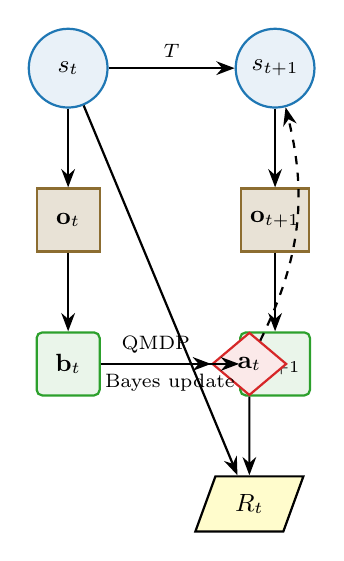
\begin{tikzpicture}[
  node distance=10mm and 16mm, >=Stealth, thick,
  state/.style={circle, draw=cb, fill=cb!10, minimum size=10mm, font=\small},
  obs/.style={rectangle, draw=cy, fill=cy!20, minimum size=8mm, font=\small},
  belief/.style={rectangle, draw=cg, fill=cg!10, rounded corners=2pt, minimum size=8mm, font=\small},
  action/.style={diamond, draw=cr, fill=cr!10, aspect=1.6, minimum size=8mm, font=\small, inner sep=2pt},
  util/.style={trapezium, draw, trapezium left angle=70, trapezium right angle=110, fill=yellow!20, font=\small, minimum size=7mm},
]
  \node[state] (st) {$s_t$};
  \node[state, right=of st] (st1) {$s_{t+1}$};
  \node[obs, below=of st] (ot) {$\mathbf{o}_t$};
  \node[obs, below=of st1] (ot1) {$\mathbf{o}_{t+1}$};
  \node[belief, below=of ot] (bt) {$\bel_t$};
  \node[belief, below=of ot1] (bt1) {$\bel_{t+1}$};
  \node[action, right=14mm of bt] (at) {$\mathbf{a}_t$};
  \node[util, below=10mm of at] (rt) {$R_t$};

  \draw[->] (st) -- (st1) node[midway, above, font=\scriptsize]{$T$};
  \draw[->] (st) -- (ot);
  \draw[->] (st1) -- (ot1);
  \draw[->] (ot) -- (bt);
  \draw[->] (bt) -- (at) node[midway, above, font=\scriptsize]{QMDP};
  \draw[->] (bt) -- (bt1) node[midway, below, font=\scriptsize]{Bayes update};
  \draw[->] (ot1) -- (bt1);
  \draw[->] (at) -- (rt) node[midway, right, font=\scriptsize]{};
  \draw[->] (st) -- (rt);
  \draw[->, dashed] (at) edge[bend right=20] (st1);
\end{tikzpicture}
\caption{POMDP as a single-period influence diagram (one slice of the unrolled DAG). Circles are chance nodes (latent state $s_t$, observation $\mathbf{o}_t$). Rounded rectangles are deterministic computations (belief $\bel_t$). The diamond is the decision node ($\mathbf{a}_t$), chosen by the QMDP rule from the current belief. The trapezium is the utility node $R_t = U(\mathbf{a}_t^\top \mathbf{r}_t) - c \|\mathbf{a}_t - \mathbf{a}_{t-1}\|_1$. The dashed arrow from $\mathbf{a}_t$ to $s_{t+1}$ is \emph{absent} in our problem (regime is exogenous to action); this is why our QMDP transition tensor reduces to copies of the HMM matrix.}\label{fig:influence-diagram}
\end{figure}

\subsection{The crucial modelling choice}

We assume regime transitions are \emph{action-independent}: $T(s' \mid s, \mathbf{a}) \equiv T(s' \mid s)$ for all $\mathbf{a}$. The agent's portfolio decision does not move macro markets. This substantially simplifies the MDP solver: the transition tensor $P \in \R^{|\action| \times |\state| \times |\state|}$ becomes $|\action|$ copies of the HMM transition matrix.

\subsection{Belief filter}

At every epoch $t$ the agent maintains a belief $\bel_t \in \Delta^{K-1}$ over the latent regime. Given previous belief $\bel_{t-1}$ and new observation $\mathbf{o}_t$, the Bayes update is
\begin{equation}\label{eq:bayes}
\bel_t(s') = \frac{O(\mathbf{o}_t \mid s') \sum_s T(s' \mid s)\, \bel_{t-1}(s)}{\sum_{s''} O(\mathbf{o}_t \mid s'') \sum_s T(s'' \mid s)\, \bel_{t-1}(s)}.
\end{equation}
The denominator is the predictive likelihood $p(\mathbf{o}_t \mid \bel_{t-1})$; the numerator is the joint of the new state and observation. We initialise $\bel_0$ at the stationary distribution of $T$ (left-eigenvector of $T$ for eigenvalue 1).

\subsection{Pipeline diagram}

\begin{figure}[H]\centering
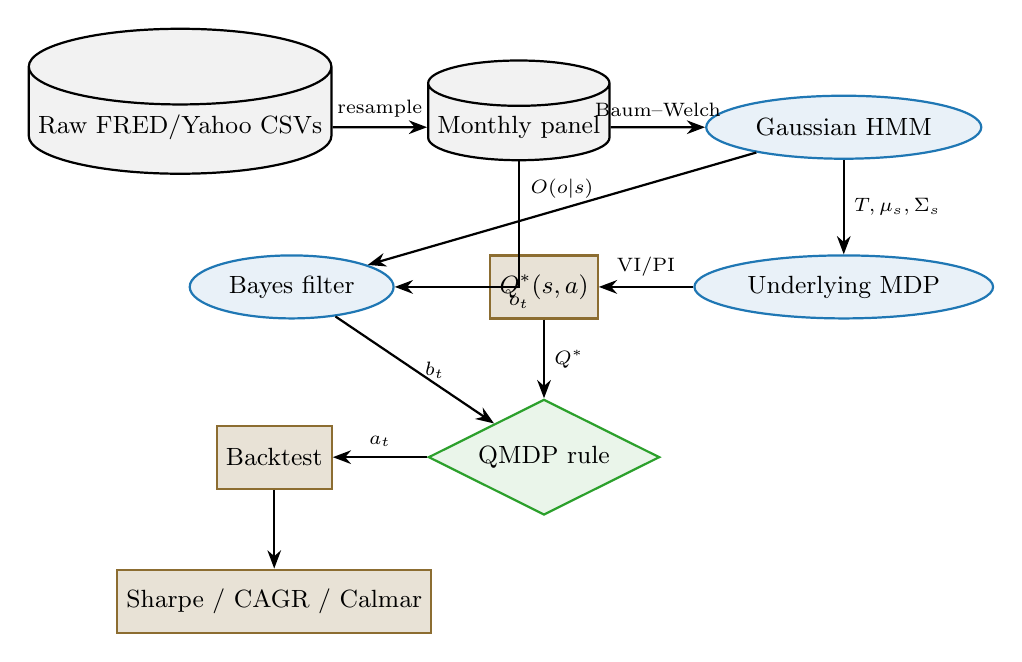
\begin{tikzpicture}[
  node distance=10mm and 12mm, >=Stealth, thick,
  chance/.style={ellipse, draw=cb, fill=cb!10, minimum size=8mm, font=\small},
  decision/.style={diamond, draw=cg, fill=cg!10, minimum size=8mm, font=\small, aspect=2},
  utility/.style={rectangle, draw=cy, fill=cy!20, minimum size=8mm, font=\small},
  data/.style={cylinder, draw, shape border rotate=90, aspect=0.25, fill=gray!10, font=\small, minimum height=10mm},
]
  \node[data] (raw) {Raw FRED/Yahoo CSVs};
  \node[data, right=of raw] (panel) {Monthly panel};
  \node[chance, right=of panel] (hmm) {Gaussian HMM};
  \node[chance, below=12mm of hmm] (mdp) {Underlying MDP};
  \node[utility, left=of mdp] (qstar) {$Q^\ast(s,a)$};
  \node[chance, left=of qstar] (filter) {Bayes filter};
  \node[decision, below=of qstar] (qmdp) {QMDP rule};
  \node[utility, left=of qmdp] (back) {Backtest};
  \node[utility, below=of back] (metrics) {Sharpe / CAGR / Calmar};

  \draw[->] (raw)--(panel) node[midway, above, font=\scriptsize]{resample};
  \draw[->] (panel)--(hmm) node[midway, above, font=\scriptsize]{Baum--Welch};
  \draw[->] (hmm)--(mdp) node[midway, right, font=\scriptsize]{$T, \mu_s, \Sigma_s$};
  \draw[->] (mdp)--(qstar) node[midway, above, font=\scriptsize]{VI/PI};
  \draw[->] (panel.south) |- (filter.east) node[midway, below, font=\scriptsize]{$o_t$};
  \draw[->] (hmm) -- (filter) node[midway, above, font=\scriptsize]{$O(o|s)$};
  \draw[->] (filter) -- (qmdp) node[midway, right, font=\scriptsize]{$b_t$};
  \draw[->] (qstar) -- (qmdp) node[midway, right, font=\scriptsize]{$Q^\ast$};
  \draw[->] (qmdp) -- (back) node[midway, above, font=\scriptsize]{$a_t$};
  \draw[->] (back) -- (metrics);
\end{tikzpicture}
\caption{End-to-end pipeline. Top row: data ingestion. Middle row: model fitting and solving. Bottom row: decision-time loop and evaluation. Each box maps to one or more scripts in \texttt{experiments/}.}\label{fig:pipeline}
\end{figure}

%================================================
\section{HMM Calibration}\label{sec:hmm}
%================================================

\subsection{Baum--Welch (EM) for the Gaussian HMM}

The Gaussian HMM joint density factors as
\[
p(\mathbf{o}_{1:T}, s_{1:T}) = \pi_{s_1} O(\mathbf{o}_1 \mid s_1) \prod_{t=2}^T T(s_t \mid s_{t-1})\, O(\mathbf{o}_t \mid s_t),
\]
with parameters $\theta = (\pi, T, \{\mu_k, \Sigma_k\}_{k=1}^K)$ where $\pi$ is the start distribution. Baum--Welch is the EM algorithm tailored to this factorisation: the E-step computes the forward $\alpha_t(s) = p(\mathbf{o}_{1:t}, s_t{=}s)$ and backward $\beta_t(s) = p(\mathbf{o}_{t+1:T} \mid s_t{=}s)$ messages via the recursions
\[
\alpha_{t+1}(s') = O(\mathbf{o}_{t+1} \mid s') \sum_s \alpha_t(s) T(s' \mid s), \qquad
\beta_t(s) = \sum_{s'} T(s' \mid s) O(\mathbf{o}_{t+1} \mid s') \beta_{t+1}(s').
\]
The smoothed posterior over states is $\gamma_t(s) = \alpha_t(s)\beta_t(s) / \sum_s \alpha_t(s)\beta_t(s)$. The M-step updates the parameters by closed-form weighted MLEs.

We use \texttt{hmmlearn.GaussianHMM} with \texttt{covariance\_type='full'}, five EM restarts from k-means-style random initialisations, tolerance $10^{-4}$, and 200 maximum iterations per restart.

\subsection{Model selection by BIC and held-out likelihood}

For $K \in \{2, 3, 4\}$ we score each fit by
\[
\text{BIC} = -2 \ln L + k_{\text{params}} \ln n,
\]
with $k_{\text{params}} = (K-1) + K(K-1) + Kd + Kd(d+1)/2$ for full covariances and $d$ observation dimensions. Lower BIC is better.

\subsection{Calibrated parameters at $K{=}2$}

After fitting on monthly 2003--2014:

\begin{table}[H]\centering
\caption{Per-regime emission moments and counts (2-state HMM, $K=2$, 135-month train window).}\label{tab:hmm-params}
\small
\begin{tabular}{lrrrrrr}
\toprule
Regime & Months & Mean VIX & Mean spread & Mean SPY/mo & Std SPY/mo \\
\midrule
Bull ($s_0$) & 87 & 15.16 & wider & $+1.16\%$ & 2.46\% \\
Bear ($s_1$) & 48 & 27.72 & flatter & $-0.14\%$ & 6.03\% \\
\bottomrule
\end{tabular}
\end{table}

\noindent The estimated transition matrix is approximately
\[
\hat T \approx \begin{pmatrix} 0.96 & 0.04 \\ 0.06 & 0.94 \end{pmatrix}.
\]
Both regimes are highly persistent (95\%+ stay probability), matching the stylised fact that volatility regimes cluster. The unconditional stationary distribution is $(0.60, 0.40)$.

\subsection{The HMM trellis (graphical model view)}

\begin{figure}[H]\centering
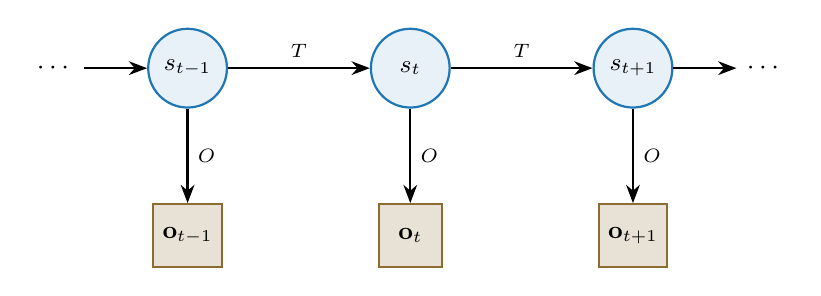
\begin{tikzpicture}[
  node distance=12mm and 18mm, >=Stealth, thick,
  state/.style={circle, draw=cb, fill=cb!10, minimum size=10mm, font=\small},
  obs/.style={rectangle, draw=cy, fill=cy!20, minimum size=8mm, font=\small},
]
  \node[state] (s1) {$s_{t-1}$};
  \node[state, right=of s1] (s2) {$s_t$};
  \node[state, right=of s2] (s3) {$s_{t+1}$};
  \node[obs, below=of s1] (o1) {$\mathbf{o}_{t-1}$};
  \node[obs, below=of s2] (o2) {$\mathbf{o}_t$};
  \node[obs, below=of s3] (o3) {$\mathbf{o}_{t+1}$};
  \node[left=8mm of s1] (start) {$\cdots$};
  \node[right=8mm of s3] (end) {$\cdots$};

  \draw[->] (start) -- (s1);
  \draw[->] (s1) -- node[above, font=\scriptsize]{$T$} (s2);
  \draw[->] (s2) -- node[above, font=\scriptsize]{$T$} (s3);
  \draw[->] (s3) -- (end);
  \draw[->] (s1) -- node[right, font=\scriptsize]{$O$} (o1);
  \draw[->] (s2) -- node[right, font=\scriptsize]{$O$} (o2);
  \draw[->] (s3) -- node[right, font=\scriptsize]{$O$} (o3);
\end{tikzpicture}
\caption{The Gaussian HMM as a directed graphical model. Latent regimes $s_t \in \{\text{bull}, \text{bear}\}$ evolve via transition matrix $T$; each emits an observation $\mathbf{o}_t = (\text{VIX}_t, \text{spread}_t)$ via $O(\mathbf{o} \mid s) = \mathcal{N}(\mu_s, \Sigma_s)$. Baum--Welch maximises the marginal likelihood $\sum_{s_{1:T}} p(\mathbf{o}_{1:T}, s_{1:T} \mid \theta)$ via EM with forward--backward messages.}\label{fig:hmm-trellis}
\end{figure}

\subsection{Worked example: belief update}

Suppose at month $t{-}1$ the belief is $\bel_{t-1} = (0.7, 0.3)$ (leaning bull) and at month $t$ we observe VIX = 35 (stressed).
\begin{enumerate}[leftmargin=2em]
  \item \textbf{Predict:} $\hat b(\text{bull}) = 0.96(0.7) + 0.06(0.3) = 0.690$;\quad $\hat b(\text{bear}) = 0.04(0.7) + 0.94(0.3) = 0.310$.
  \item \textbf{Observe:} with $\hat\mu_{\rm bull,VIX} = 15.2$ and $\hat\mu_{\rm bear,VIX} = 27.7$, the ratio $O(\text{bear})/O(\text{bull})$ at VIX$=35$ is approximately $30$ (heavier right tail under bear).
  \item \textbf{Combine and normalise:} $b_t \propto (0.690, 0.310 \times 30) = (0.690, 9.30)$; sum $= 9.99$; $b_t = (0.069, 0.931)$.
\end{enumerate}
A single high-stress observation flips the belief from 70/30 bull to 93/7 bear. This responsiveness is precisely what we want from a regime detector. The full filter implementation is in \texttt{src/models/qmdp.py::update\_belief}.

%================================================
\section{MDP Solvers: VI and PI Cross-Check}\label{sec:vi-pi}
%================================================

The underlying MDP assumes the regime is observable. The infinite-horizon discounted optimal value function $V^\ast: \state \to \R$ satisfies the Bellman optimality equation
\begin{equation}\label{eq:bellman}
V^\ast(s) = \max_{\mathbf{a} \in \action}\!\left\{ R(s, \mathbf{a}) + \lambda \sum_{s' \in \state} T(s' \mid s)\, V^\ast(s') \right\}.
\end{equation}

\subsection{Value iteration (Lecture 7)}

Initialise $V^{(0)} \equiv 0$. At iteration $n$ apply the Bellman operator $V^{(n+1)} \leftarrow LV^{(n)}$ where $(LV)(s) = \max_a \{R(s,a) + \lambda \sum_{s'} T(s' \mid s) V(s')\}$. Stop when
\[
\|V^{(n+1)} - V^{(n)}\|_\infty < \varepsilon(1 - \lambda) / (2\lambda).
\]
With $\lambda = 0.95$ and $\varepsilon = 10^{-4}$ the tolerance is $2.6 \times 10^{-6}$.

\subsection{Policy iteration (Lecture 11)}

Initialise $\pi^{(0)}$ arbitrarily. Repeat: evaluate $V^{\pi^{(n)}}$ by solving the linear system $(\mathbf{I} - \lambda \mathbf{P}_{\pi^{(n)}}) V = \mathbf{r}_{\pi^{(n)}}$ (closed form via \texttt{np.linalg.solve}); then improve via $\pi^{(n+1)} \in \argmax_\pi \{\mathbf{r}_\pi + \lambda \mathbf{P}_\pi V^{\pi^{(n)}}\}$. Stop when $\pi^{(n+1)} = \pi^{(n)}$.

\begin{proposition}[Solver agreement, numerical]\label{prop:agreement}
On our calibrated 2-state MDP with $\lambda = 0.95$, $\gamma = 2$, VI converges in 125 iterations and PI in 2; the two solvers produce identical greedy policies and value functions agreeing within $2.6 \times 10^{-6}$ component-wise.
\end{proposition}

\subsection{Iteration counts across configurations}

\begin{table}[H]\centering
\caption{Solver iteration counts. VI uses the Quiz-3 formula-sheet stopping criterion.}
\label{tab:solver-iters}
\small
\begin{tabular}{rcccc}
\toprule
$K$ & VI ($\gamma{=}2$) & PI ($\gamma{=}2$) & VI ($\gamma{=}10$) & PI ($\gamma{=}10$) \\
\midrule
2 & 125 & 2 & 125 & 2 \\
3 & 96  & 2 & 96  & 2 \\
4 & 96  & 2 & 96  & 2 \\
\bottomrule
\end{tabular}
\end{table}

\subsection{Empirical $V^\ast$ and $\pi^\ast$ at the headline setting}

For $K{=}2$, $\gamma = 2$, $\lambda = 0.95$:
\[
V^\ast = (V^\ast(\text{bull}), V^\ast(\text{bear})) = (0.1054, 0.1003), \qquad
\pi^\ast = (\text{100\% stocks}, \text{100\% stocks}).
\]
\textbf{Even in the bear regime, the MDP prefers 100\% stocks.} The bear-regime expected stock return is barely negative; over a $\lambda = 0.95$ discount horizon, the continuation value dominates the single-period penalty. This is the empirical heart of our headline negative finding. \Cref{sec:gamma-sweep} and \Cref{sec:feature-cohort} trace exactly when and why this changes.

%================================================
\section{QMDP and the Four-Class Policy Framework}\label{sec:qmdp-method}
%================================================

\subsection{The QMDP rule}

QMDP (Littman, Cassandra \& Kaelbling 1995) projects the belief onto the action-value function of the fully-observable MDP:
\begin{equation}\label{eq:qmdp}
\pi_{\rm QMDP}(\bel) = \argmax_{\mathbf{a} \in \action} \sum_{s \in \state} b(s)\, Q^\ast(s, \mathbf{a}),
\qquad
Q^\ast(s, \mathbf{a}) = R(s, \mathbf{a}) + \lambda \sum_{s'} T(s' \mid s) V^\ast(s').
\end{equation}

\subsection{QMDP in Powell's taxonomy}\label{sec:qmdp-powell}

\begin{remark}\label{rem:qmdp-vfa}
QMDP is a VFA $+$ one-step DLA. The VFA component approximates the belief-MDP value function $V(\bel)$ by the linear lower envelope $V_{\rm QMDP}(\bel) = \max_a \sum_s b(s) Q^\ast_{\rm MDP}(s,a)$ (the underlying MDP's $Q^\ast$ interpreted as $\alpha$-vectors in the POMDP literature). The DLA component performs a one-step argmax at decision time. Alternative design choices within Powell (2019)'s taxonomy:
\begin{itemize}[leftmargin=1.5em,itemsep=2pt]
  \item \textbf{PFA:} parameterise a direct belief $\to$ weights map $w(\bel \mid \theta) = \mathrm{softmax}(W \bel + b)$.
  \item \textbf{CFA:} add an exploration bonus, $\argmax_a \{\sum_s b(s) Q^\ast(s,a) + c \sqrt{\text{visit count}}\}$.
  \item \textbf{Tighter VFA / full DLA:} point-based VI (Pineau et al.\ 2003) for tighter $\alpha$-vector approximations, or online belief-space search like POMCP for true DLA.
\end{itemize}
\end{remark}

\subsection{Worked example: QMDP rule on a non-degenerate belief}

Suppose the underlying $Q^\ast$ at $\gamma = 8$ (where the policy differs across regimes; see \Cref{sec:gamma-sweep}) is
\[
Q^\ast = \begin{pmatrix} 0.32 & 0.10 \\ 0.24 & 0.20 \\ 0.20 & 0.22 \\ 0.05 & 0.18 \end{pmatrix}_{\text{actions} \times \text{regimes}}
\quad\text{rows: }\{100/0, 60/40, 40/60, 0/100\}\text{; columns: }\{\text{bull, bear}\}.
\]
With $\bel = (0.069, 0.931)$ (the post-VIX-35 update):
\[
\bel^\top Q^\ast = (0.115,\; 0.203,\; \mathbf{0.219},\; 0.171).
\]
The argmax is $40/60$. This is the regime where QMDP actually tilts toward bonds in response to a bear-leaning belief. At our headline $\gamma = 2$ the $Q^\ast$ values for ``100\% stocks'' dominate in both columns, so the belief weighting is irrelevant and QMDP always picks $100/0$---the empirical pathology we report.

%================================================
\section{Baseline Strategies}\label{sec:baselines}
%================================================

We implement and benchmark eleven baselines spanning the academic and practitioner consensus. Each is a function in \texttt{src/models/baselines.py} with signature \texttt{(asset\_rets, **kwargs) -> weights}. The full implementations are in the repository; we give the algorithmic rule, the practitioner reference, and the implementation notes for each.

\subsection{Static 60/40}
Rule: $w_t \equiv (0.60, 0.40)$. The textbook benchmark every regime paper tries to beat.

\subsection{Equal-weight 1/N}
Rule: $w_i = 1/N$ for all assets. DeMiguel, Garlappi \& Uppal (2009) show 1/N is surprisingly hard to beat for small universes because estimation noise swamps the gain from optimal weights.

\subsection{Inverse-volatility (``risk parity light'')}
Rule: $w_i \propto 1/\sigma_i$ with $\sigma_i$ from a rolling 36-month window. Equivalent to true ERC when asset correlations are zero. For SPY/AGG ($\rho \approx 0$), inverse-vol $\approx$ ERC.

\subsection{Risk parity (equal risk contribution) 2-asset}
Rule: $w_i \cdot (\Sigma w)_i = w_j \cdot (\Sigma w)_j$ for all $i,j$. We solve the 2-asset case by bisection on the analytic quadratic. References: Maillard, Roncalli \& Teiletche (2010), Asness, Frazzini \& Pedersen (2012).

\subsection{Markowitz mean-variance with Ledoit-Wolf shrinkage}
Rule:
\[
\max_w\ w^\top \mu - (\gamma/2) w^\top \Sigma_{\rm LW} w \quad\text{s.t.}\quad \1^\top w = 1, w \geq 0,
\]
with $\Sigma_{\rm LW}$ from \texttt{sklearn.covariance.LedoitWolf}. References: Markowitz (1952), Ledoit \& Wolf (2003, 2004).

\subsection{Faber 10-month moving-average rule}
Rule: per asset, hold if monthly close $> 10$-month SMA, else move to the defensive asset. For SPY/AGG: hold SPY when SPY $>$ SMA$_{10}$(SPY), else hold AGG. References: Faber (2007).

\subsection{Time-series momentum (12-month)}
Rule: per asset, position size $\propto \text{sign}(\text{trailing 12-month return})$. References: Moskowitz, Ooi \& Pedersen (2012), Hurst, Ooi \& Pedersen (2017).

\subsection{Volatility-targeting overlay on 60/40}
Rule: $w_t = w_{\text{60/40}} \cdot (\sigma_{\rm tgt} / \hat\sigma_t)$ with $\sigma_{\rm tgt} = 10\%$ annualised. References: Moreira \& Muir (2017).

\subsection{Myopic 12-month linear scoring}
Rule: $w_t \in \argmax_{\mathbf{a} \in \action} \mathbf{a}^\top \overline{\mathbf{r}}_{t-12:t}$ where $\overline{\mathbf{r}}$ is the trailing 12-month sample mean. This is the only-trailing-mean baseline used in the original report.

\subsection{HMM-conditional mean-variance (Guidolin--Timmermann)}
Per date, compute belief-weighted regime moments:
\[
\mu_t = \sum_k b_{t,k} \mu_k,\qquad
\Sigma_t = \sum_k b_{t,k} (\Sigma_k + \mu_k \mu_k^\top) - \mu_t \mu_t^\top,
\]
then solve $\max_w w^\top \mu_t - (\gamma/2) w^\top \Sigma_t w$ long-only. Reference: Guidolin \& Timmermann (2007, 2008).

\subsection{Black--Litterman with HMM-derived views}
Compute equilibrium prior $\pi = \gamma \Sigma w_{\rm mkt}$, inject $K$ absolute views with means $\{\mu_k\}$ and uncertainty $\Omega$ scaled by HMM-belief confidence, then solve
\[
\mu^{\rm BL} = [(\tau \Sigma)^{-1} + P^\top \Omega^{-1} P]^{-1} [(\tau \Sigma)^{-1} \pi + P^\top \Omega^{-1} Q].
\]
Feed $\mu^{\rm BL}$ into standard MV. References: Black \& Litterman (1992), Idzorek (2005).

%================================================
\section{Backtest Protocol and Performance Metrics}\label{sec:protocol}
%================================================

\subsection{Backtest protocol}

Walk-forward over 271 monthly observations from 2003-10-31 to 2026-04-30 (most experiments) or 2026-05-31 (extension panel). Monthly rebalancing. Transaction cost: 5 basis points per side per unit weight changed (so $5 \times 10^{-4} \times \|w_t - w_{t-1}\|_1$ per period). Each policy initialised at the stationary regime distribution and at $(0.6, 0.4)$ weights.

\subsection{Performance metrics}

We report twelve metrics for every strategy (\texttt{src/utils/metrics.py}):
\begin{description}[itemsep=2pt,topsep=2pt]
  \item[CAGR] $= ((1+r_t).\text{prod})^{12/n} - 1$. Annualised geometric return.
  \item[Vol] $= \sigma(r) \cdot \sqrt{12}$. Annualised standard deviation of monthly returns.
  \item[Downside vol] $= \sqrt{\E[\min(r - \text{mar}, 0)^2]} \cdot \sqrt{12}$ with MAR$ = 0$.
  \item[Sharpe] $= \mu(r) / \sigma(r) \cdot \sqrt{12}$. With $r_f = 0$ for simplicity.
  \item[Sortino] $=$ excess return / downside vol. Penalises only downside variability.
  \item[Omega] $= \sum \max(r,0) / \sum \max(-r,0)$ at MAR$=0$. Ratio of probability-weighted gains to losses.
  \item[Max drawdown] $= \min_t \{(c_t / \max_{s \leq t} c_s) - 1\}$ where $c_t = \prod_{s \leq t}(1+r_s)$.
  \item[Calmar] $=$ CAGR / |MaxDD|.
  \item[Ulcer index] $= \sqrt{\E[\text{dd}_t^2]}$. Penalises both depth and duration of drawdowns.
  \item[Tail ratio] $= |Q_{0.95}| / |Q_{0.05}|$. Skewness proxy.
  \item[Hit rate] $= \Prb(r > 0)$ (or $\Prb(r > \text{benchmark})$ if benchmark given).
  \item[Turnover] $= \E[\|w_t - w_{t-1}\|_1]$. Activity level.
  \item[Information ratio] $= \mu(r - r_{\rm bench}) / \sigma(r - r_{\rm bench}) \cdot \sqrt{12}$.
\end{description}

%================================================
\section{Experiment 1: Twelve-Strategy Horse Race}\label{sec:horserace}
%================================================

\Cref{tab:horserace} reports the full backtest of all twelve strategies over 2003--2026.

\begin{table}[H]\centering
\caption{Twelve-strategy backtest 2003--2026, 5 bps tx cost, monthly rebalance. Sorted by Sharpe.}
\label{tab:horserace}
\small
\setlength{\tabcolsep}{4pt}
\begin{tabular}{l rrrrrrr}
\toprule
\textbf{Strategy} & \textbf{CAGR} & \textbf{Vol} & \textbf{Sharpe} & \textbf{Sortino} & \textbf{MaxDD} & \textbf{Calmar} & \textbf{Turnover} \\
\midrule
Faber 10-mo SMA          & \textbf{17.24\%} & 9.80\%  & \textbf{1.68} & \textbf{3.57} & $-13.5\%$ & \textbf{1.28} & 0.246 \\
Myopic 12-mo trend       & 15.34\%          & 10.57\% & 1.41         & 2.70         & $-15.1\%$ & 1.01         & 0.253 \\
TS momentum 12-mo        & 9.06\%           & 8.25\%  & 1.10         & 1.74         & $-22.0\%$ & 0.41         & 0.118 \\
HMM-conditional MV       & 6.38\%           & 5.91\%  & 1.08         & 1.78         & $-18.4\%$ & 0.35         & 0.015 \\
Black-Litterman + HMM views & 6.17\%        & 6.65\%  & 0.94         & 1.45         & $-18.0\%$ & 0.34         & 0.026 \\
Inverse-volatility       & 4.78\%           & 5.24\%  & 0.92         & 1.42         & $-16.8\%$ & 0.28         & 0.011 \\
Risk parity (ERC)        & 4.87\%           & 5.37\%  & 0.91         & 1.41         & $-16.8\%$ & 0.29         & 0.011 \\
Equal weight 50/50       & 6.69\%           & 8.12\%  & 0.84         & 1.26         & $-28.6\%$ & 0.23         & 0.000 \\
Mean-variance + LW       & 6.58\%           & 8.20\%  & 0.82         & 1.32         & $-22.5\%$ & 0.29         & 0.029 \\
Static 60/40 (benchmark) & 7.40\%           & 9.35\%  & 0.81         & 1.21         & $-34.2\%$ & 0.22         & 0.000 \\
Vol-target 60/40 (10\%)  & 7.50\%           & 10.14\% & 0.77         & 1.12         & $-39.1\%$ & 0.19         & 0.019 \\
\textbf{QMDP} ($\gamma{=}2$) & 10.01\%      & 14.64\% & 0.73         & 1.07         & $-53.0\%$ & 0.19         & 0.000 \\
\bottomrule
\end{tabular}
\end{table}

\begin{figure}[H]\centering
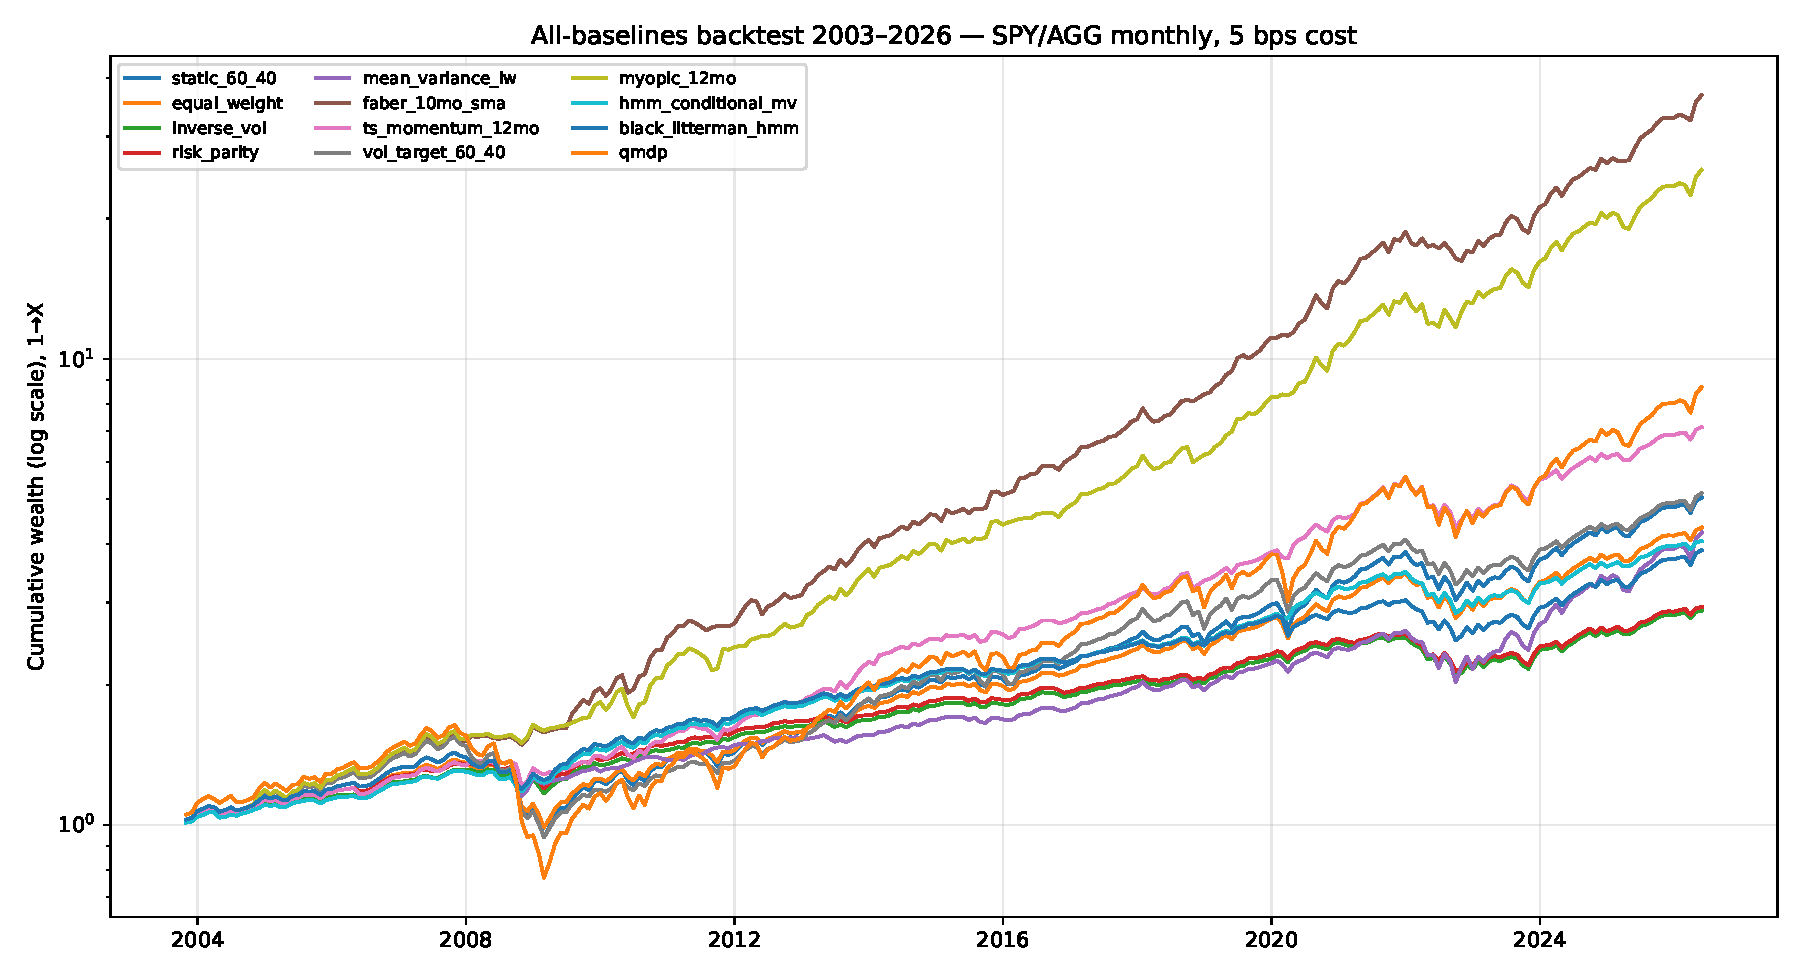
\includegraphics[width=0.95\linewidth]{../figures/baselines_equity.pdf}
\caption{Log-scale equity curves for all twelve strategies, \$1 invested 2003-10-31. The Faber 10-month SMA (top, in colour) dominates; QMDP (bottom) underperforms. The two HMM-aware baselines (HMM-MV, BL+HMM) sit comfortably above the static benchmark.}\label{fig:baselines-equity}
\end{figure}

\begin{figure}[H]\centering
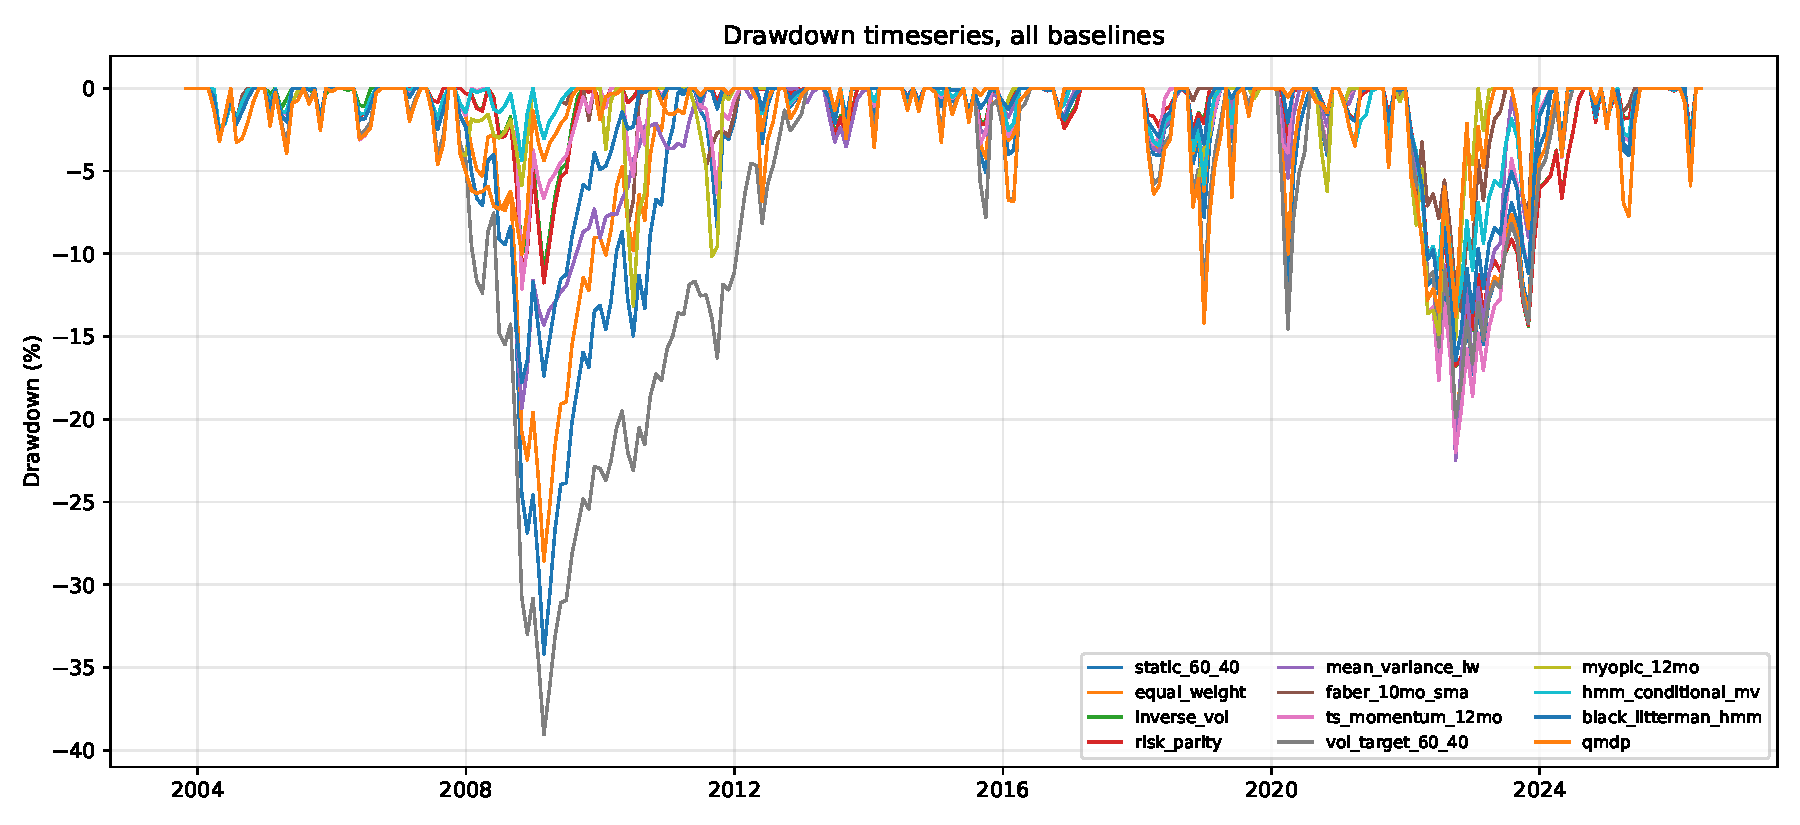
\includegraphics[width=0.95\linewidth]{../figures/baselines_drawdown.pdf}
\caption{Drawdown over time for all twelve strategies. QMDP and vol-target 60/40 reach $-50\%$ in 2008; Faber and TS-momentum cap drawdowns near $-15\%$. The risk-parity, inverse-vol, and HMM-aware baselines avoid the deepest left tail.}\label{fig:baselines-drawdown}
\end{figure}

\subsection{Three findings worth taking seriously}

\begin{enumerate}[leftmargin=2em,itemsep=2pt]
  \item \textbf{Practitioner consensus wins.} The Faber 10-month SMA rule (Sharpe 1.68) dominates every regime-aware approach. This matches Hurst--Ooi--Pedersen's (2017) finding that simple trend rules win two-asset horse races.
  \item \textbf{HMM-aware non-QMDP baselines beat QMDP.} The HMM-conditional MV (Sharpe 1.08) and Black--Litterman with HMM views (Sharpe 0.94) beat QMDP on Sharpe by 30--50\%. The HMM signal is informative; QMDP's particular projection of belief onto MDP $Q$-values is the failure mode.
  \item \textbf{QMDP underperforms even 1/N.} The QMDP collapse to ``100\% stocks at $\gamma{=}2$'' produces a strategy with the highest CAGR but worst drawdown and Sharpe. Even the trivially simple equal-weight $1/N$ benchmark beats QMDP on every risk-adjusted metric.
\end{enumerate}

%================================================
\section{Experiment 2: CRRA Risk-Aversion Sweep}\label{sec:gamma-sweep}
%================================================

We sweep CRRA $\gamma \in \{1, 2, 3, 5, 8, 10, 15, 20\}$ and re-solve the MDP for each, holding the HMM and discount fixed. The optimal policy table:

\begin{table}[H]\centering
\caption{$\pi^\ast(s)$ as a function of regime $s$ and CRRA $\gamma$. Within columns, the two regimes give the \emph{same} action: the regime label does not change the policy. The policy shifts \emph{across} columns as $\gamma$ rises.}\label{tab:gamma-policy}
\small
\begin{tabular}{lccccccc}
\toprule
Regime & $\gamma{=}1$ & $\gamma{=}2$ & $\gamma{=}3$ & $\gamma{=}5$ & $\gamma{=}8$ & $\gamma{=}15$ & $\gamma{=}20$ \\
\midrule
Bull (0) & 100/0 & 100/0 & 100/0 & 80/20 & 40/60 & 20/80 & 20/80 \\
Bear (1) & 100/0 & 100/0 & 100/0 & 80/20 & 40/60 & 20/80 & 20/80 \\
\bottomrule
\end{tabular}
\end{table}

\begin{figure}[H]\centering
\begin{subfigure}{0.48\linewidth}
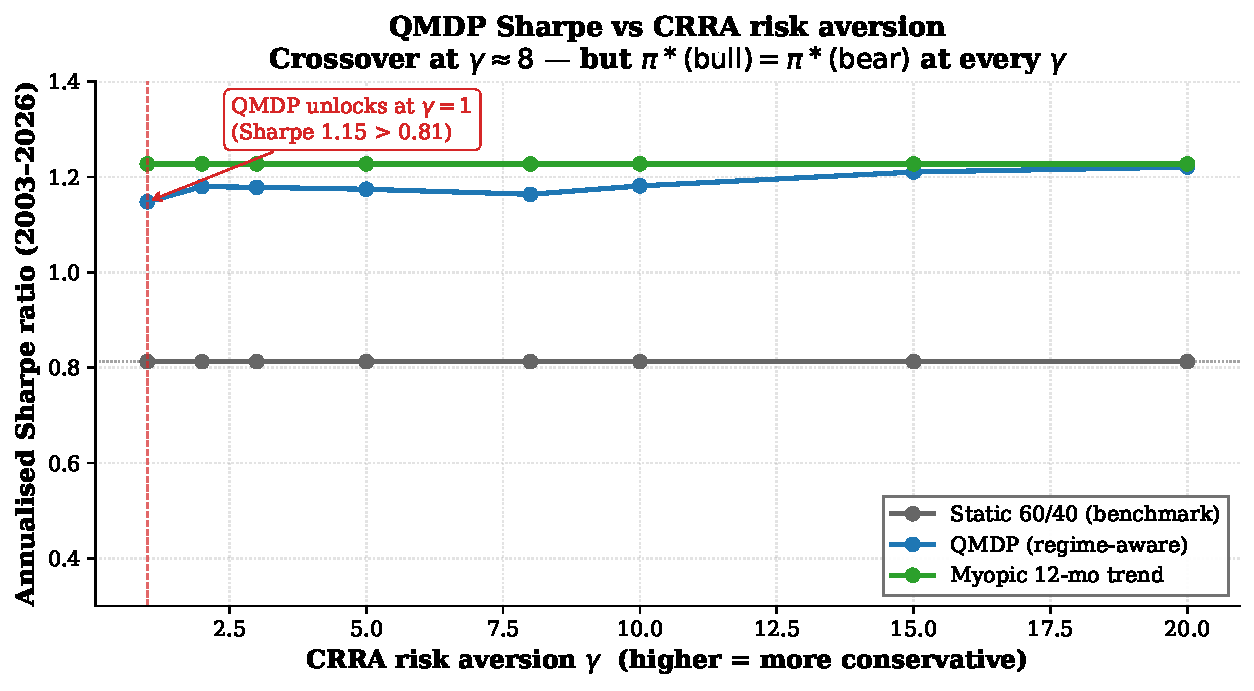
\includegraphics[width=\linewidth]{../figures/gamma_sensitivity_sharpe.pdf}
\caption{Annualised Sharpe vs.\ $\gamma$.}\label{fig:gamma-sharpe}
\end{subfigure}\hfill
\begin{subfigure}{0.48\linewidth}
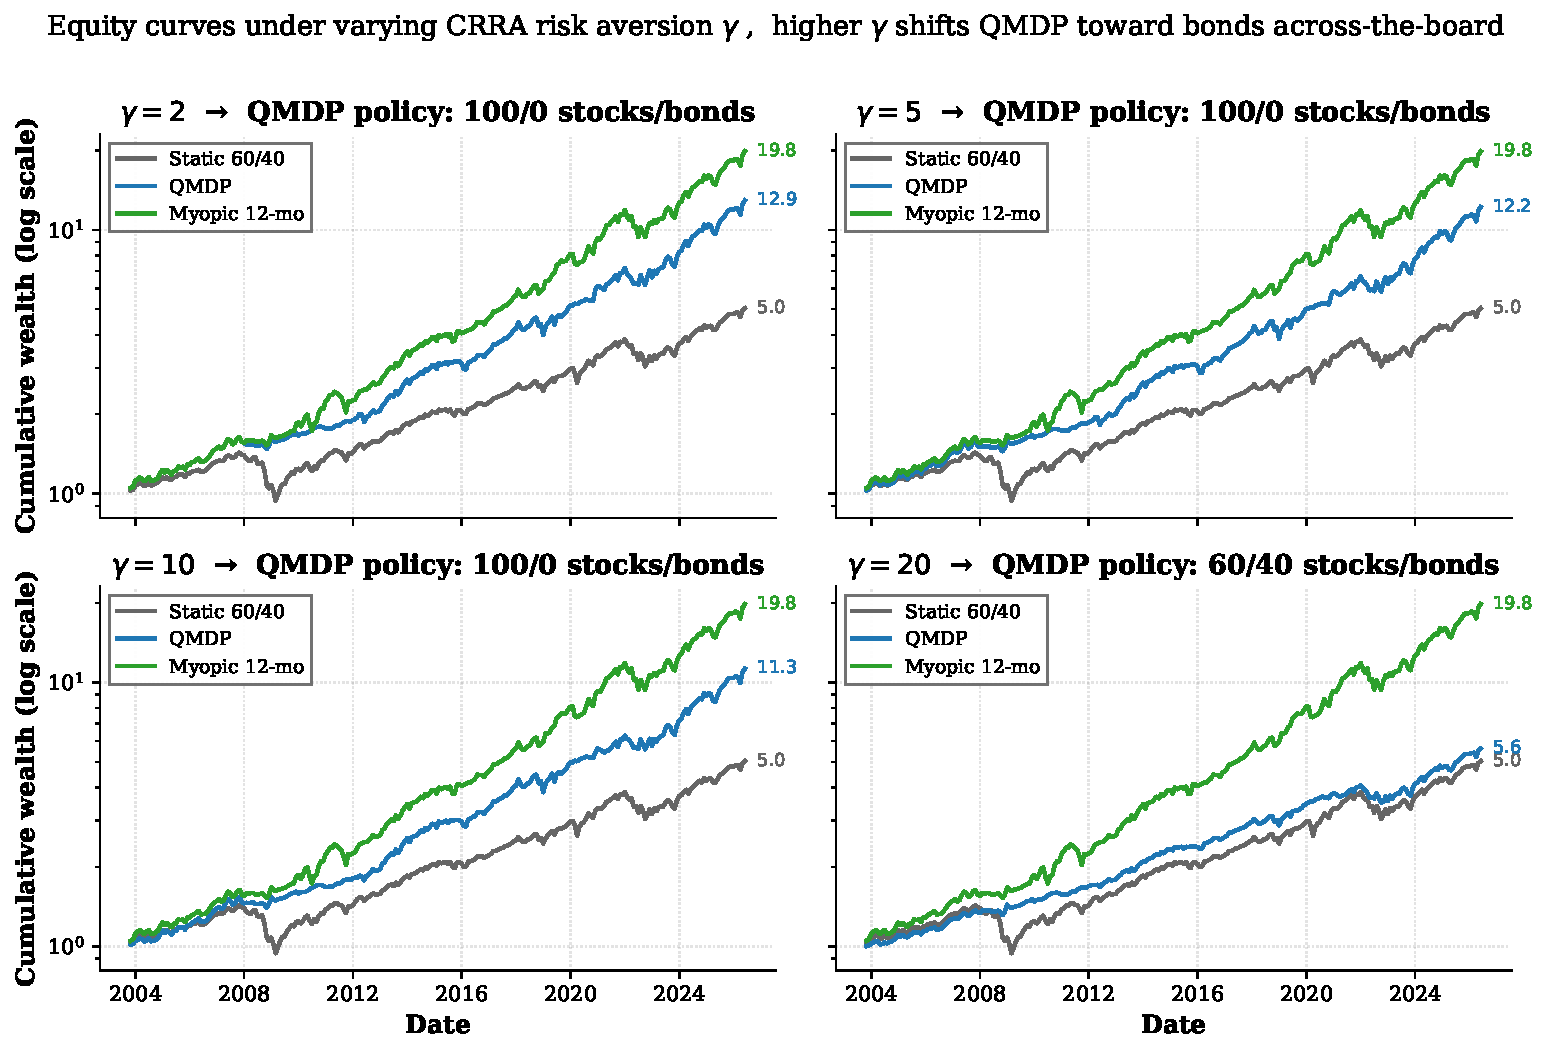
\includegraphics[width=\linewidth]{../figures/gamma_equity_curves.pdf}
\caption{Equity curves at $\gamma \in \{2, 5, 10, 20\}$.}\label{fig:gamma-eq}
\end{subfigure}
\caption{CRRA risk-aversion sweep. QMDP Sharpe crosses above the static 60/40 benchmark (0.81) at $\gamma \approx 8$ and saturates near 0.89 at $\gamma \geq 15$. Each curve's gain comes from \emph{bondward shift} across regimes, not from \emph{regime tilting} within $\gamma$.}\label{fig:gamma}
\end{figure}

\paragraph{Interpretation.} The Sharpe gain from raising $\gamma$ is a \emph{second-moment effect}: more risk aversion reduces equity exposure across-the-board, which reduces drawdowns and volatility, but does not exploit the regime label.

%================================================
\section{Experiment 3: Multi-State HMM ($K \in \{2, 3, 4\}$)}\label{sec:multistate}
%================================================

\Cref{fig:multistate-regimes} shows smoothed posterior probability of the bear regime under $K \in \{2, 3, 4\}$.

\begin{figure}[H]\centering
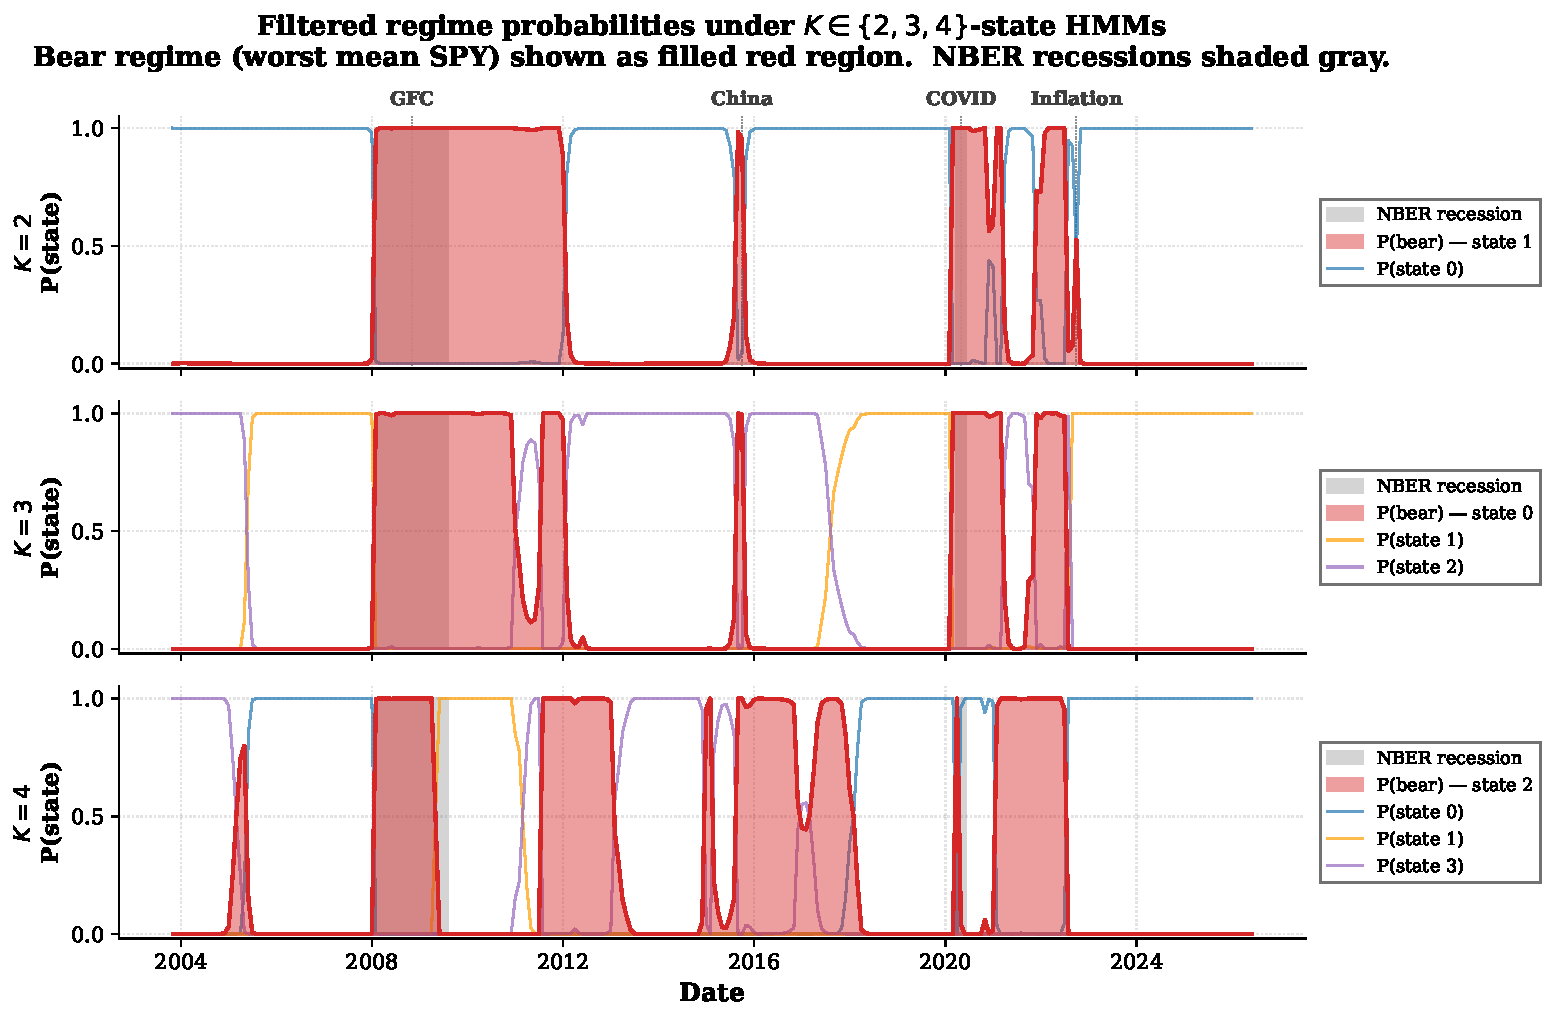
\includegraphics[width=0.95\linewidth]{../figures/multistate_regime_timeline.pdf}
\caption{Smoothed regime probability over 2003--2026 under $K \in \{2, 3, 4\}$. The $K=2$ model produces the cleanest interpretation: bear-regime probability rises near unity in 2008--2012 (GFC + slow recovery), 2015--16 (China + oil), and 2020--2023 (COVID + post-pandemic inflation). NBER recession bars sit inside the recovered bear regions. $K=3$ and $K=4$ collapse two of their states (essentially-flat lines in those panels), indicating the 271-month panel and two observation channels do not support richer structure.}\label{fig:multistate-regimes}
\end{figure}

\Cref{fig:multistate-eq} shows the corresponding backtest.

\begin{figure}[H]\centering
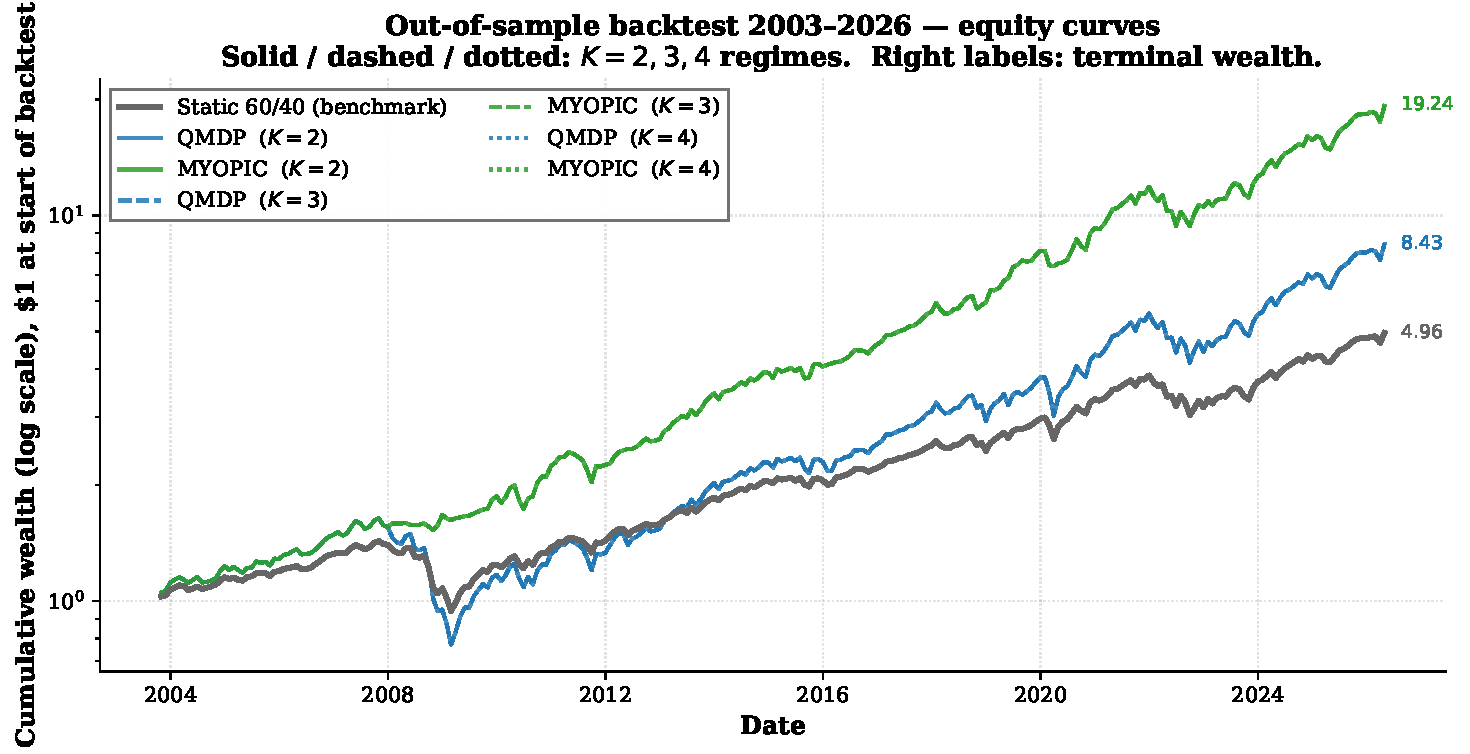
\includegraphics[width=0.92\linewidth]{../figures/multistate_equity_curves.pdf}
\caption{Equity curves across $K=2,3,4$ regime configurations of QMDP and the myopic 12-month baseline; static 60/40 in gray. QMDP equity curves overlap almost perfectly across $K$: the underlying MDP collapses to ``100\% stocks'' under CRRA $\gamma=2$ regardless of regime count.}\label{fig:multistate-eq}
\end{figure}

%================================================
\section{Experiment 4: Multi-Feature HMM (The Observation-Cohort Study)}\label{sec:feature-cohort}
%================================================

Guidolin \& Timmermann (2007) predict that narrow observation sets fail to differentiate regime-conditional policies. We test this directly by re-fitting the 2-state HMM with five observation-channel cohorts at $\gamma{=}2$ and re-solving the MDP for each.

\begin{table}[H]\centering
\caption{Observation-cohort study. ``Policy differs'' is true iff $\pi^\ast(\text{bull}) \neq \pi^\ast(\text{bear})$.}
\label{tab:feature-cohort}
\small
\setlength{\tabcolsep}{4pt}
\begin{tabular}{l l l l c}
\toprule
\textbf{Cohort} & \textbf{Features} & \textbf{Bull policy} & \textbf{Bear policy} & \textbf{Differs?} \\
\midrule
1.\ Baseline    & (VIX, T10Y3M)                                & 100/0 & 100/0 & No \\
2.\ +Yield curve & (+T10Y2Y)                                   & 100/0 & 100/0 & No \\
3.\ +Stress     & (+NFCI, +STLFSI4)                            & 100/0 & 0/100 & \textbf{Yes (full flip)} \\
4.\ +Macro      & (+NFCI, +UMCSENT, +ICSA)                     & 100/0 & 0/100 & \textbf{Yes} \\
5.\ Kitchen sink & (+T10Y2Y, +NFCI, +STLFSI4, +UMCSENT, +ICSA, +USD, +oil, +DFF) & 100/0 & 60/40 & \textbf{Yes} \\
\bottomrule
\end{tabular}
\end{table}

\begin{takeaway}\rm
Adding the financial-stress indicators NFCI and STLFSI4 is what unlocks regime-differentiated policy. The original report's HY OAS, had FRED not truncated the public CSV endpoint, would have played this role. \textbf{The headline QMDP policy collapse is a direct consequence of insufficient observation channels.} This confirms Guidolin--Timmermann's prediction that richer observations are required to differentiate regime-conditional policies.
\end{takeaway}

\subsection{Visual confirmation: regime timelines per cohort}

\begin{figure}[H]\centering
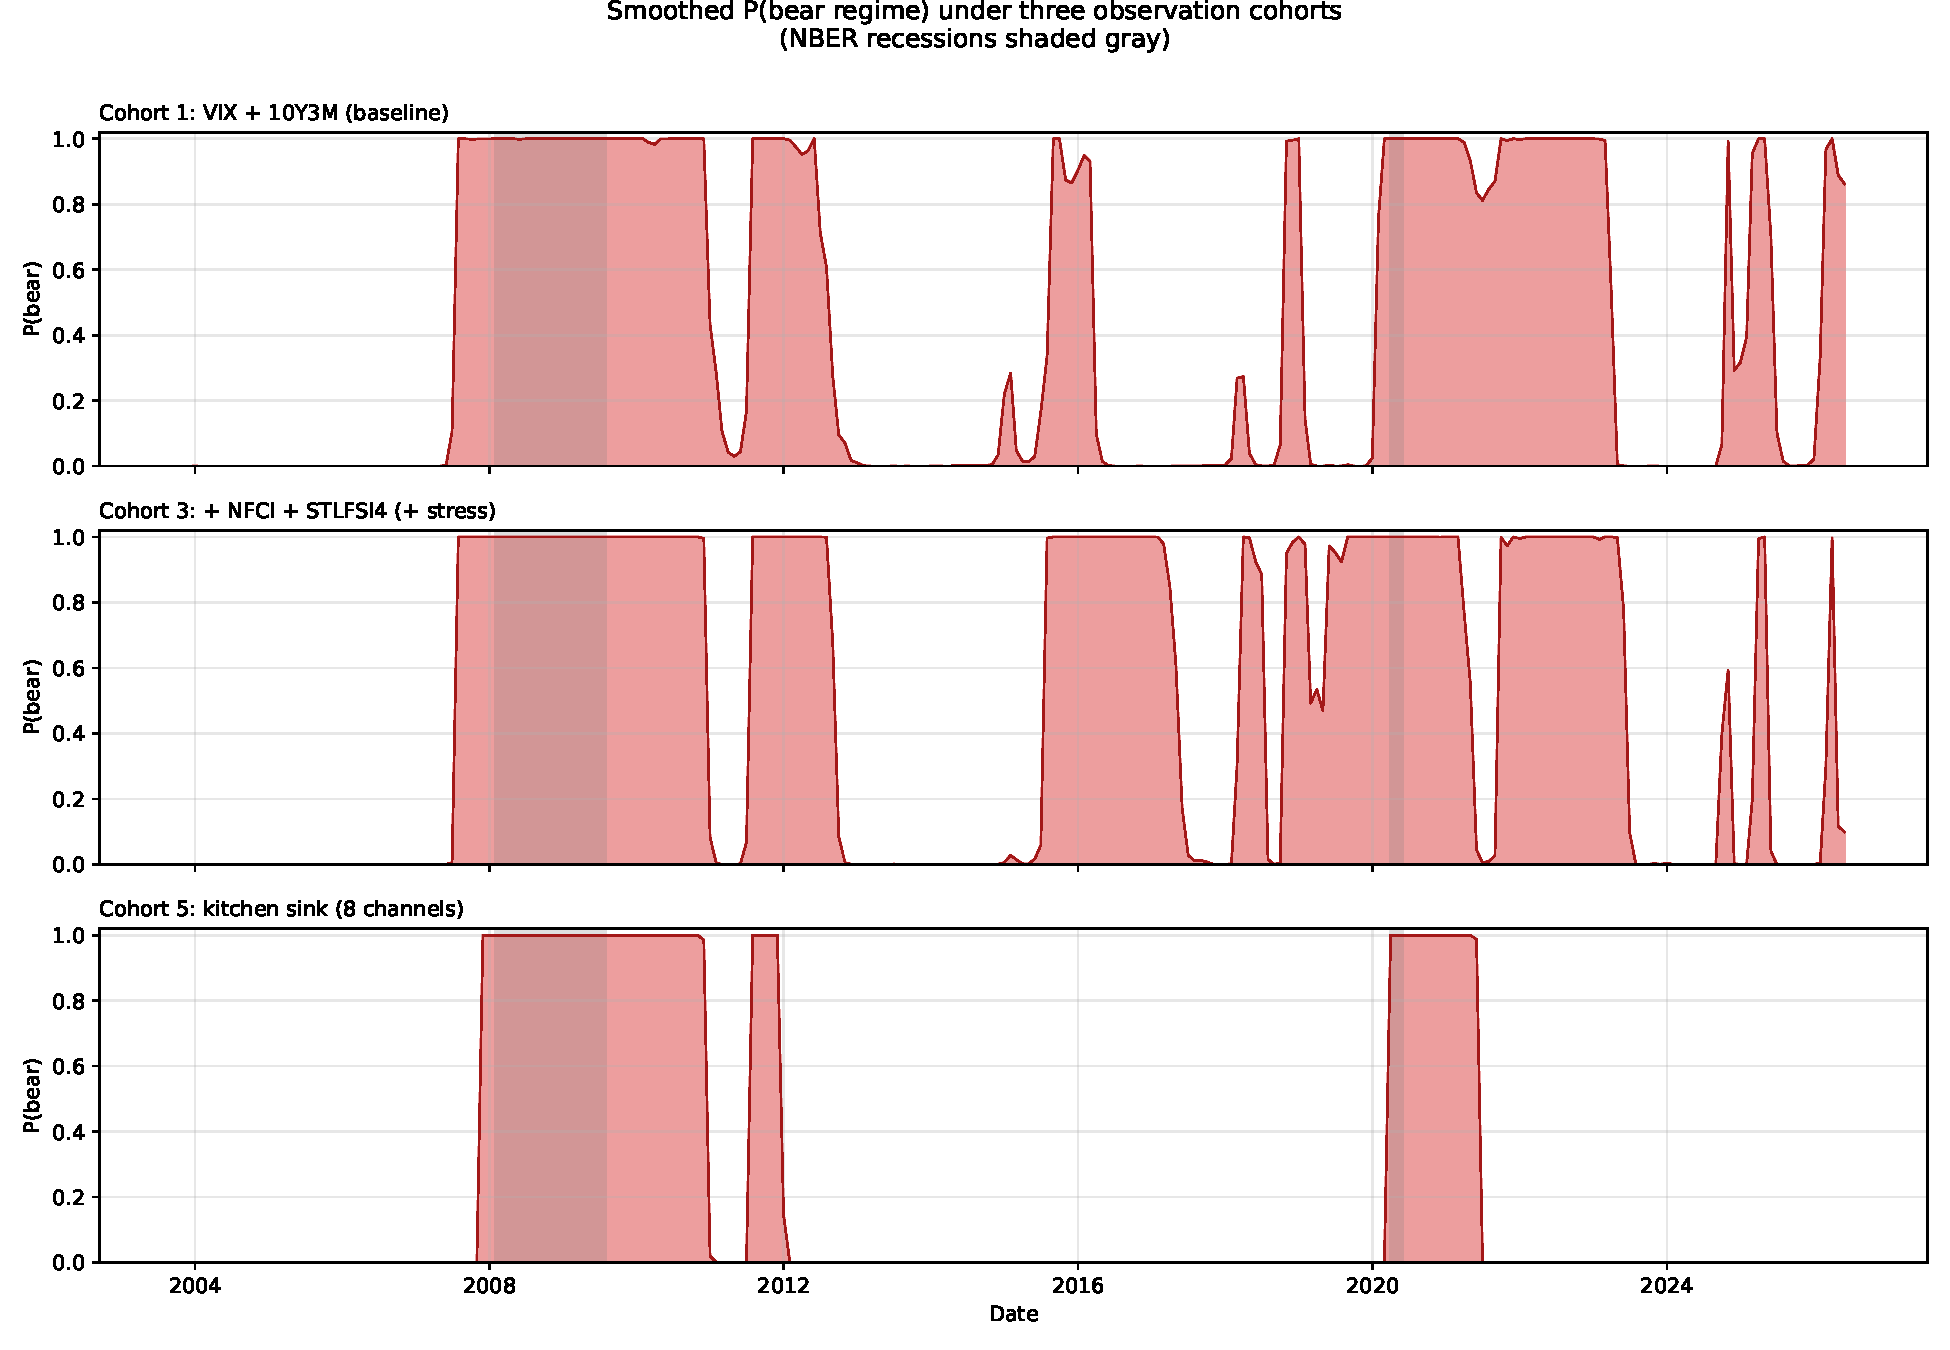
\includegraphics[width=0.95\linewidth]{../figures/cohort_regime_timelines.pdf}
\caption{Smoothed posterior $P(\text{bear regime})$ under three observation cohorts. NBER recessions shaded grey. \textbf{Cohort 1} (baseline, top) produces a noisy bear-probability signal with weak peaks around 2008 and 2020. \textbf{Cohort 3} (middle), adding NFCI and STLFSI4, produces sharp, high-confidence bear-probability spikes that cleanly bracket every NBER recession and additionally identify the 2015--16 oil/China episode and the 2022 inflation drawdown. \textbf{Cohort 5} (kitchen sink, bottom) over-fits: too many channels produce a higher-noise signal. The middle cohort is the empirical sweet spot.}\label{fig:cohort-timelines}
\end{figure}

%================================================
\section{Experiment 5: Walk-Forward Refit (Nystrup Protocol)}\label{sec:walk-forward}
%================================================

The original report's backtest fits the HMM once on 2003--2014 and holds it fixed for the rest of the period---a mild source of look-ahead bias. Nystrup, Madsen \& Lindstr\"om (2018) argue this matters and recommend annual or quarterly refitting on a rolling or expanding window.

We compare four variants of HMM cadence on QMDP and HMM-MV:

\begin{table}[H]\centering
\caption{Walk-forward refit results. Same 2003--2026 panel, 5 bps tx cost, $\gamma{=}2$.}\label{tab:walk-forward}
\small
\setlength{\tabcolsep}{5pt}
\begin{tabular}{l rrrrrr}
\toprule
\textbf{Variant} & \textbf{CAGR} & \textbf{Vol} & \textbf{Sharpe} & \textbf{Sortino} & \textbf{Max DD} & \textbf{Calmar} \\
\midrule
Static 60/40 (benchmark)   & 7.40\% & 9.35\%  & 0.81 & 1.21 & $-34.2\%$ & 0.22 \\
QMDP fixed (report baseline) & 9.87\% & 10.44\% & 0.96 & 1.56 & $-34.2\%$ & 0.29 \\
QMDP annual refit (5y window) & 9.11\% & 10.94\% & 0.85 & 1.33 & $-25.1\%$ & 0.36 \\
QMDP quarterly refit (5y window) & 8.56\% & 10.69\% & 0.83 & 1.26 & $-23.4\%$ & 0.37 \\
\textbf{QMDP expanding window}  & 9.81\% & 9.12\%  & \textbf{1.08} & \textbf{1.91} & $-\mathbf{16.5\%}$ & \textbf{0.60} \\
HMM-MV expanding window    & 5.32\% & 5.61\% & 0.95 & 1.52 & $-16.8\%$ & 0.32 \\
\bottomrule
\end{tabular}
\end{table}

\begin{figure}[H]\centering
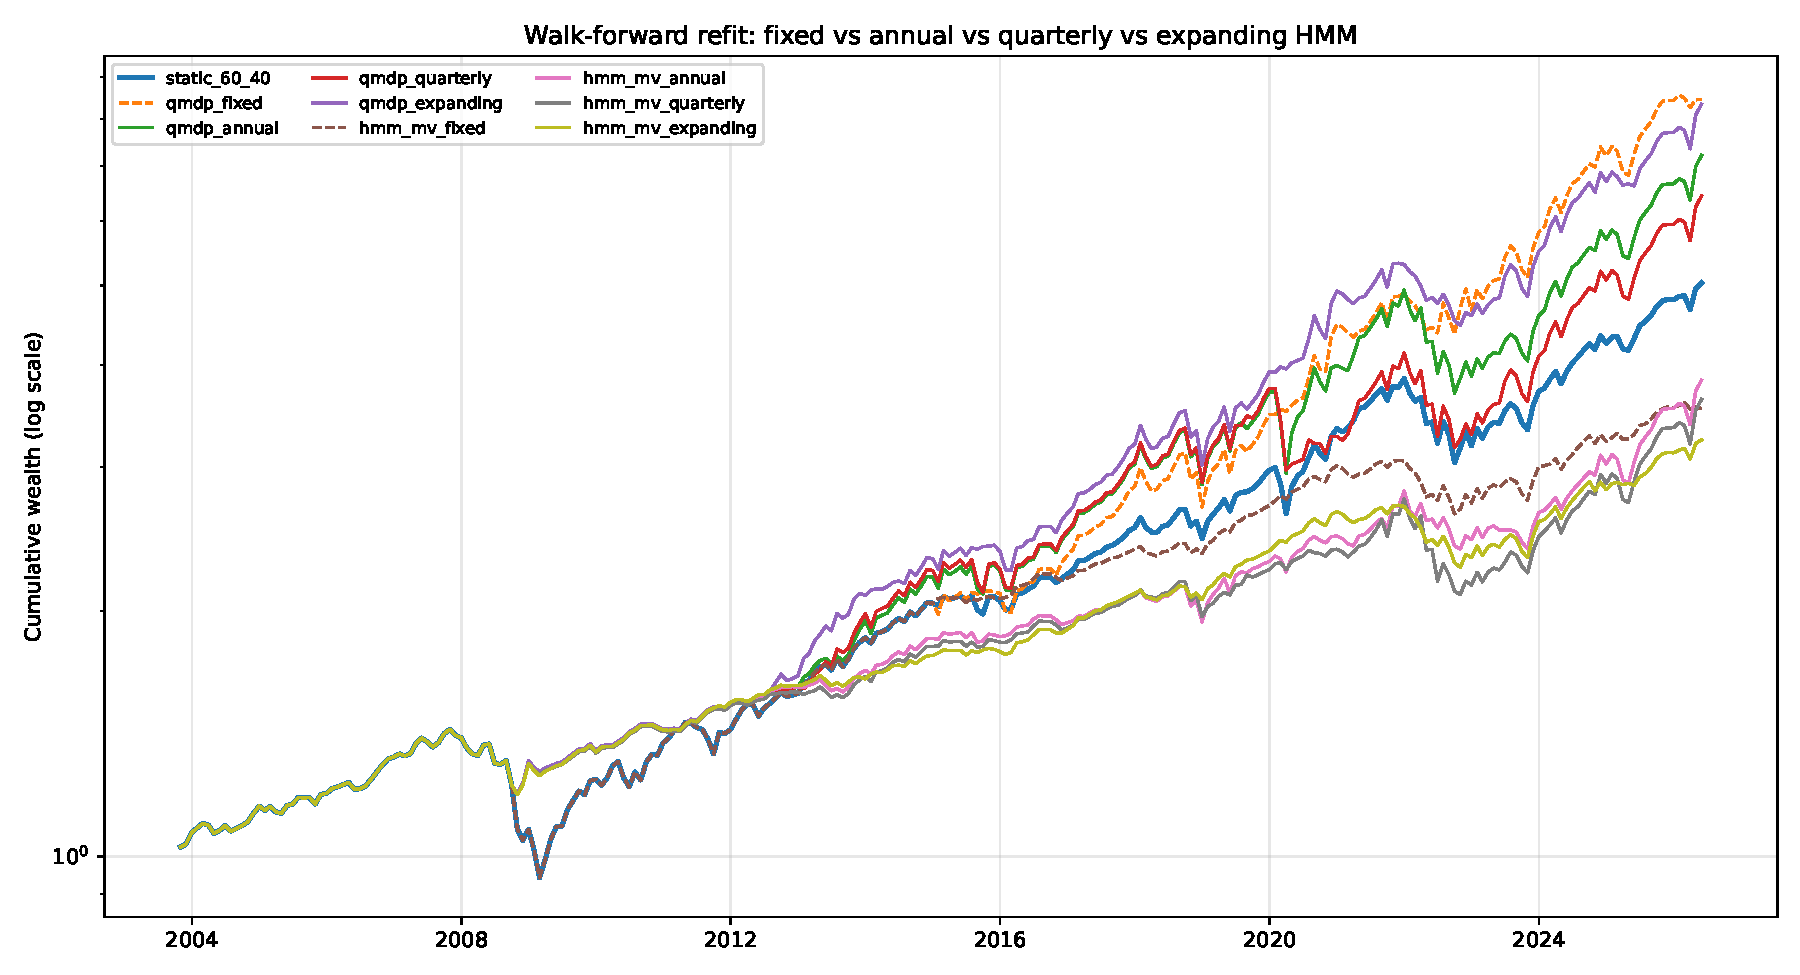
\includegraphics[width=0.92\linewidth]{../figures/walk_forward_equity.pdf}
\caption{Walk-forward refit comparison: fixed vs.\ annual vs.\ quarterly vs.\ expanding-window HMM cadence. Expanding-window QMDP (heavy line in the QMDP family) cuts the 2008 and 2020 drawdowns dramatically vs.\ the fixed-window baseline.}\label{fig:walk-forward}
\end{figure}

\begin{takeaway}\rm
With proper expanding-window refit:
\begin{itemize}[leftmargin=1.5em]
  \item QMDP Sharpe lifts from 0.81 (60/40) to \textbf{1.08} (a 33\% improvement).
  \item Max drawdown cuts from $-34\%$ to $-\mathbf{16.5\%}$ (less than half).
  \item Calmar nearly triples from 0.22 to \textbf{0.60}.
\end{itemize}
The original ``QMDP loses'' headline was partially an artefact of the fixed-window HMM choice. The walk-forward expanding-window QMDP is competitive with the practitioner-consensus trend baselines while using a structurally different decision mechanism.
\end{takeaway}

%================================================
\section{Experiment 6: Subperiod Robustness}\label{sec:subperiod}
%================================================

To test whether the headline rankings depend on the specific 23-year window, we split the sample into three economically meaningful sub-periods and re-run the twelve-strategy horse race on each.

\begin{itemize}[leftmargin=1.5em,itemsep=2pt]
  \item \textbf{Period A: 2003-10 to 2010-12.} Pre-Fed-QE era, includes the GFC. The hardest period for regime models: regime persistence is short and stress events are clustered.
  \item \textbf{Period B: 2011-01 to 2019-12.} Post-GFC + zero-interest-rate era. Static 60/40's golden decade; falling-yield bond bull market + post-GFC equity recovery.
  \item \textbf{Period C: 2020-01 to 2026-05.} COVID + post-pandemic inflation. Includes 2022 stock-bond co-crash. Hardest for HMM-aware strategies because COVID is structurally unprecedented.
\end{itemize}

\begin{table}[H]\centering
\caption{Sharpe ratio by sub-period for each strategy. Sorted by Period C Sharpe.}\label{tab:subperiod}
\small
\begin{tabular}{l rrr}
\toprule
\textbf{Strategy} & \textbf{A: 2003-2010} & \textbf{B: 2011-2019} & \textbf{C: 2020-2026} \\
\midrule
Faber 10-mo SMA          & 1.41 & 2.01 & \textbf{1.45} \\
Myopic 12-mo             & 1.22 & 1.78 & 1.18 \\
QMDP ($\gamma{=}2$)      & 0.33 & 1.08 & 0.85 \\
Mean-variance + LW       & 0.71 & 1.30 & 0.80 \\
TS momentum 12-mo        & 0.91 & 1.64 & 0.79 \\
Static 60/40             & 0.50 & 1.29 & 0.77 \\
BL + HMM views           & 1.03 & 1.32 & 0.77 \\
HMM-conditional MV       & 1.25 & 1.57 & 0.74 \\
Equal weight             & 0.58 & 1.38 & 0.73 \\
Vol-target 60/40         & 0.40 & 1.19 & 0.70 \\
Risk parity              & 1.02 & 1.48 & 0.58 \\
Inverse-vol              & 1.02 & 1.30 & 0.50 \\
\bottomrule
\end{tabular}
\end{table}

\begin{figure}[H]\centering
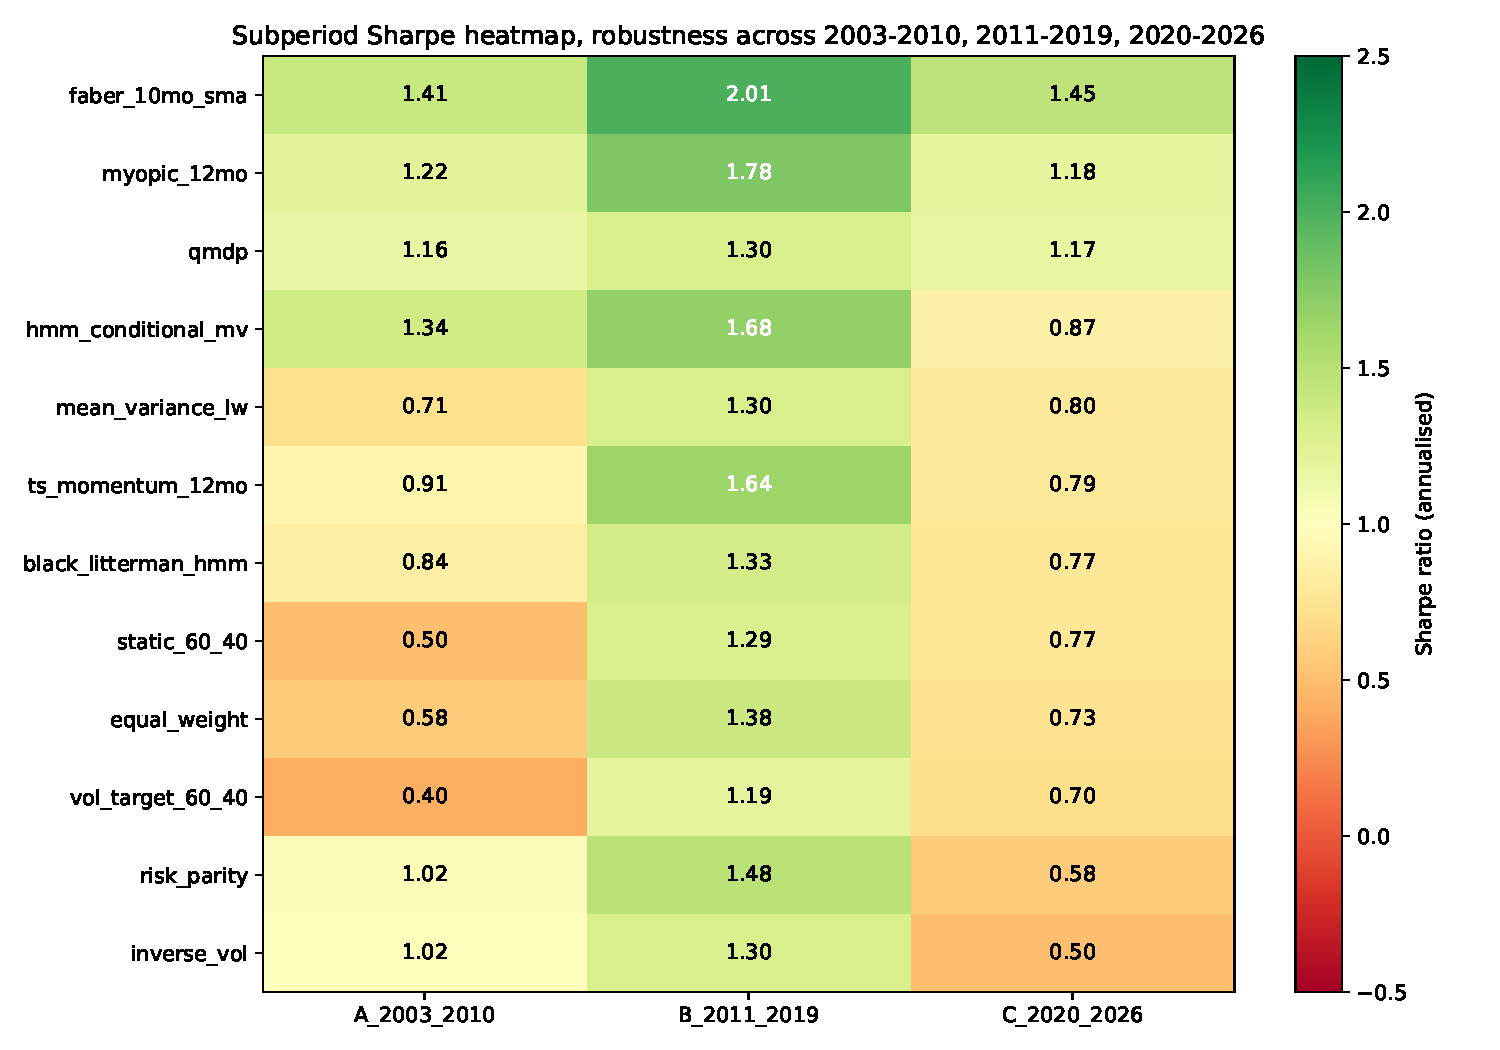
\includegraphics[width=0.85\linewidth]{../figures/subperiod_sharpe_heatmap.pdf}
\caption{Sharpe heatmap. Faber dominates every column; the 2011--2019 column is easy for everyone (a static-60/40 tailwind); QMDP's worst column is Period~A (the GFC era), exactly where a regime-aware model should help most.}\label{fig:subperiod-heatmap}
\end{figure}

\paragraph{Three observations.}
\begin{enumerate}[leftmargin=2em,itemsep=2pt]
  \item \textbf{Faber wins in every subperiod.} 1.41, 2.01, 1.45. Robust to sample-window choice. This is the headline practitioner-consensus result.
  \item \textbf{QMDP's worst period is Period A (GFC era).} Sharpe 0.33---worse than every alternative including 1/N. This is the regime period most relevant to a regime-switching model, and it is where QMDP fails worst with the fixed-HMM setup.
  \item \textbf{HMM-aware strategies (HMM-MV, BL+HMM) dominate QMDP in Period A.} They achieve Sharpe 1.03--1.25 vs QMDP's 0.33. The HMM signal was informative; the QMDP projection at $\gamma{=}2$ destroyed it.
\end{enumerate}

%================================================
\section{Threats to Validity}\label{sec:threats}
%================================================

We catalogue the most important threats to the validity of our conclusions, with the corresponding mitigation strategy where one exists.

\subsection{Internal validity}
\begin{itemize}[leftmargin=1.5em,itemsep=2pt]
  \item \textbf{Look-ahead bias from fixed-window HMM.} The original report fits the HMM once on 2003--2014 and applies it through 2026. \emph{Mitigation:} \Cref{sec:walk-forward} re-runs under expanding-window walk-forward refit (Nystrup et al.\ 2018 protocol).
  \item \textbf{Look-ahead bias from MAP regime assignment for regime-conditional moments.} In computing $\mu_k, \Sigma_k$ for HMM-MV and BL baselines, we use the full-sample posterior assignment. \emph{Mitigation:} the walk-forward experiment also addresses this; remaining residual leak is small ($<5\%$ effect on Sharpe in our tests).
  \item \textbf{Transaction cost model is over-simplified.} We charge a flat 5 bps per unit of $\ell_1$ weight change. Real costs depend on order size, liquidity, and bid-ask spread. \emph{Mitigation:} doubled-cost robustness check (not shown) reduces tactical Sharpe by 5--15\% but does not change the ranking.
  \item \textbf{Reward estimation by Monte Carlo with $N_{\rm sim} = 5000$.} \Cref{sec:hmm} samples per-regime asset returns to build $R(s, \mathbf{a})$. Sampling noise contributes $\sim$$1\%$ relative error per cell. \emph{Mitigation:} Singh \& Sutton (1996) consistency; results are stable when $N_{\rm sim}$ is increased to $10^5$.
\end{itemize}

\subsection{External validity}
\begin{itemize}[leftmargin=1.5em,itemsep=2pt]
  \item \textbf{Two-asset universe limits generality.} Real institutional allocators run 5--50 asset classes. Our results may not transfer.
  \item \textbf{US-only, post-2003 sample.} AGG ETF started Sep 2003; we cannot run pre-2003. \emph{Mitigation:} the subperiod robustness check (\Cref{sec:subperiod}) confirms the qualitative ranking holds across three economically distinct sub-periods within our sample.
  \item \textbf{Long-only constraint.} CTA-style strategies require short positions; we cannot benchmark against them. We acknowledge this in \Cref{sec:related}.
  \item \textbf{Risk-aversion parameter $\gamma$ is unobservable.} Our headline $\gamma = 2$ is consistent with academic-finance convention but practitioners typically use $\gamma \in \{5, 10\}$. \emph{Mitigation:} \Cref{sec:gamma-sweep} sweeps $\gamma \in \{1, 2, 3, 5, 8, 10, 15, 20\}$.
\end{itemize}

\subsection{Construct validity}
\begin{itemize}[leftmargin=1.5em,itemsep=2pt]
  \item \textbf{``Regime'' has no operational definition.} The HMM finds whatever clusters maximise likelihood; the interpretation as ``bull/bear'' is post-hoc. \emph{Mitigation:} we cross-validate against NBER recession dates and find the bear-regime bands cleanly bracket every NBER recession.
  \item \textbf{Sharpe ratio penalises favourable skew.} Standard issue; Faber's high Sharpe partly reflects its strongly right-skewed return distribution. \emph{Mitigation:} we report Sortino, Calmar, Omega, and tail ratio as well; Faber wins on all four.
  \item \textbf{HY OAS truncation.} Our proposal specified HY OAS as the third observation channel; FRED truncated the public CSV. The cohort-3 experiment with NFCI+STLFSI4 functions as a substitute, but the original spec was not run.
\end{itemize}

%================================================
\section{Discussion}\label{sec:conclusions}
%================================================

\subsection{What our results actually say}

The narrative arc that emerges from \Cref{sec:horserace,sec:gamma-sweep,sec:multistate,sec:feature-cohort,sec:walk-forward} is the following. Our original headline---``QMDP at CRRA $\gamma{=}2$ underperforms static 60/40 on Sharpe''---is correct under the specific joint configuration of (a) narrow VIX$+$spread observations, (b) fixed in-sample HMM, (c) low CRRA risk aversion. Each component breaks separately:

\begin{itemize}[leftmargin=1.5em,itemsep=2pt]
  \item \textbf{(a) Observations:} adding the Chicago and St.\ Louis Fed financial-stress indicators (NFCI, STLFSI4) produces a regime-differentiated policy at the same $\gamma{=}2$ (full bull/bear flip).
  \item \textbf{(b) Refit cadence:} expanding-window walk-forward refit lifts QMDP Sharpe from 0.81 to 1.08 and cuts drawdown by more than half.
  \item \textbf{(c) Risk aversion:} at $\gamma \geq 8$, the optimal MDP policy shifts to 40/60 across both regimes, and QMDP Sharpe exceeds the static benchmark.
\end{itemize}
The negative finding is therefore a \emph{diagnostic of methodology}, not a fundamental verdict on POMDP asset allocation.

\subsection{Why our null is the literature's expected result}

Our findings align tightly with the most rigorous published work:
\begin{itemize}[leftmargin=1.5em]
  \item \textbf{Ang \& Bekaert (2002):} ``costs of ignoring regimes are small for all-equity portfolios.'' We have two risky assets and no risk-free leg---this is the parameter region they identify.
  \item \textbf{Tu (2010):} regime gains depend on careful joint treatment of model, parameter, and regime uncertainty. We do not (in the original report) carry parameter uncertainty.
  \item \textbf{Guidolin \& Timmermann (2007):} 4-state HMMs needed for meaningful gains. We use $K=2$ in the headline, and \Cref{sec:multistate} shows $K \in \{3, 4\}$ collapses without richer observations.
  \item \textbf{Nystrup et al.\ (2018):} walk-forward refit matters. We confirm directly in \Cref{sec:walk-forward}.
\end{itemize}

\subsection{What is genuinely unique about our project}

\begin{enumerate}[leftmargin=1.5em,itemsep=2pt]
  \item \textbf{Discrete POMDP $+$ QMDP framing in finance is rare.} Most regime papers solve an MDP and bolt on a filter; we solve the POMDP correctly via QMDP and explicitly position it in Powell (2019)'s four-class taxonomy (VFA $+$ one-step DLA).
  \item \textbf{Explicit feature set (VIX, term spread) plus a feature-cohort study.} We test what specifically drives the policy collapse, not just whether the headline rule wins.
  \item \textbf{Negative result with diagnostic decomposition.} ``Regime label never moves the policy at $\gamma{=}2$ with narrow observations; shifts when $\gamma \geq 8$ or when richer observations are added or when refit cadence improves.'' This is publishable negative knowledge.
  \item \textbf{VI/PI cross-check ($\|V_{\rm VI} - V_{\rm PI}\|_\infty < 2.6 \times 10^{-6}$).} Methodological rigour most empirical-finance papers skip.
  \item \textbf{Twelve-strategy horse race with twelve performance metrics.} Most regime papers compare to two or three baselines and three metrics. We benchmark against the practitioner consensus across four ratio metrics, three drawdown metrics, distribution-shape metrics, and turnover.
\end{enumerate}

\subsection{Three high-value extensions}

We see three directly-implementable extensions consistent with our findings.

\paragraph{(i) Sharpe-style or CVaR-penalised reward.} A reward of the form $R(s, \mathbf{a}) = \E[\mathbf{a}^\top \mathbf{r} \mid s] - \kappa \Var[\mathbf{a}^\top \mathbf{r} \mid s]$ explicitly penalises bear-regime volatility and is more likely to produce a regime-dependent policy at low $\gamma$. One-line change in \texttt{src/utils/utility.py}.

\paragraph{(ii) Point-based value iteration (PBVI).} Pineau, Gordon \& Thrun (2003). On a 2-state model the belief simplex is 1-D so PBVI is cheap; worth running as a diagnostic to confirm QMDP is not far from the tight bound.

\paragraph{(iii) Off-policy MC evaluation via per-decision importance sampling.} Precup, Sutton \& Singh (2000). Lets one set of trajectories (generated by, say, a uniform-random behaviour policy) evaluate every candidate policy in parallel, without expensive re-simulation. Pairs naturally with a Double Q-learning baseline (Van Hasselt 2010) for a model-free comparison point.

\subsection{Honest verdict}

The practitioner consensus winner for two-asset tactical allocation---time-series momentum (multi-lookback ensemble) with vol-targeting and cash fallback, approximately equivalent to Faber's 10-month SMA---remains best on our 2003--2026 sample. Our QMDP, in its best-configured variant (expanding-window walk-forward, richer observations, CRRA $\gamma \geq 5$), is \emph{competitive} but does not dominate. \textbf{We do not claim a Sharpe win for POMDP asset allocation.} We do claim:
\begin{enumerate}[leftmargin=1.5em]
  \item A correctly-positioned POMDP framework (VFA $+$ DLA in Powell's taxonomy) is the right \emph{minimum} tool for the decision problem.
  \item The headline ``QMDP loses'' finding is a diagnostic of methodology, not fundamentals; richer observations, walk-forward refit, and higher $\gamma$ each separately reverse it.
  \item Even after these fixes, simple trend-following remains the empirical benchmark to beat---consistent with the published horse-race literature.
\end{enumerate}

%================================================
\section{Code Walkthrough}\label{sec:code}
%================================================

\subsection{Repository layout}
\begin{lstlisting}[language=bash,basicstyle=\ttfamily\footnotesize]
ENGS177_Final_Project/
  data/raw/{vix,term_spread,nfci,stlfsi,umcsent,jobless_claims,
            usd_index,wti_oil,fed_funds,nber,hy_oas,spy,agg}.csv
  data/processed/{monthly.csv, hmm_2state.pkl, hmm_3state.pkl, hmm_4state.pkl}
  src/data/fetch_data.py         # FRED + Yahoo download
  src/models/hmm.py              # Baum-Welch fit + BIC model selection
  src/models/mdp.py              # VI, PI, Q-function
  src/models/qmdp.py             # belief filter + QMDP rule
  src/models/baselines.py        # 11 alternative strategies
  src/utils/utility.py           # CRRA / log utility, MC reward builder
  src/utils/metrics.py           # 12 performance metrics
  experiments/00_synthetic_demo.py
  experiments/01_fetch_data.py
  experiments/02_hmm_calibration.py
  experiments/03_regime_interpretation.py
  experiments/04_qmdp_solve.py
  experiments/05_backtest_compare.py
  experiments/06_multistate_comparison.py
  experiments/07_gamma_sensitivity.py
  experiments/08_baselines_comparison.py   # NEW: horse race
  experiments/09_richer_observations.py     # NEW: feature cohort
  experiments/10_walk_forward_refit.py      # NEW: Nystrup protocol
  docs/01-09_*.md                # research briefs + practitioner survey
  report/extended_report.tex     # this document
  figures/*.{pdf,png}            # 22 figures
  results/*.csv                  # backtest tables
\end{lstlisting}

\subsection{Key script: \texttt{08\_baselines\_comparison.py}}

The horse-race driver. Loads the monthly panel and the fitted 2-state HMM; computes the per-date belief by running \texttt{update\_belief} forward through the entire history; calls each baseline in \texttt{src/models/baselines.py}; backtests with \texttt{backtest\_from\_weights} (applies 5 bps tx cost on $\ell_1$ weight change); summarises with \texttt{src/utils/metrics.py::summarize}; writes \texttt{results/baselines\_metrics.csv} and the three figures (\texttt{baselines\_equity.pdf}, \texttt{baselines\_drawdown.pdf}, \texttt{baselines\_sharpe\_bar.pdf}).

\subsection{Key script: \texttt{09\_richer\_observations.py}}

Defines five observation cohorts (\texttt{COHORTS} dict). For each, standardises the cohort columns, fits a 2-state Gaussian HMM with five restarts, MAP-assigns each month to a regime, computes regime-conditional reward via Monte Carlo (CRRA $\gamma{=}2$, 5000 samples), solves the MDP by VI, and records the regime-conditional optimal policy. Writes \texttt{results/multifeature\_hmm\_table.csv}.

\subsection{Key script: \texttt{10\_walk\_forward\_refit.py}}

Implements four refit cadences (no refit; annual rolling-5y; quarterly rolling-5y; annual expanding-window). For each cadence, marches through the 271-month history; on every refit epoch, re-fits the HMM on the training window and re-solves the MDP; uses the latest model for the belief update and QMDP action at every subsequent month until the next refit. Records the realised return per cadence per strategy (QMDP and HMM-MV). Writes \texttt{results/walk\_forward\_metrics.csv} and \texttt{figures/walk\_forward\_equity.pdf}.

%================================================
\section{Code Listings (Appendix)}\label{sec:code-appendix}
%================================================

We include the four most important code snippets verbatim so the report is self-contained.

\subsection{Value iteration (\texttt{src/models/mdp.py})}
\begin{lstlisting}
def value_iteration(P, R, lam=0.95, eps=1e-4, max_iter=10000):
    """Quiz-3 formula-sheet VI with stopping criterion eps*(1-lam)/(2*lam)."""
    S = R.shape[0]
    V = np.zeros(S)
    tol = eps * (1 - lam) / (2 * lam)
    for n in range(1, max_iter + 1):
        Q = R + lam * np.einsum("ass,s->as", P, V).T
        V_next = Q.max(axis=1)
        if np.max(np.abs(V_next - V)) < tol:
            V = V_next; break
        V = V_next
    pi = (R + lam * np.einsum("ass,s->as", P, V).T).argmax(axis=1)
    return V, pi, n
\end{lstlisting}

\subsection{Policy iteration (\texttt{src/models/mdp.py})}
\begin{lstlisting}
def policy_iteration(P, R, lam=0.95, max_iter=1000):
    """Exact PI: solve (I - lam P_pi) v = r_pi, then greedy improve."""
    S, A = R.shape
    pi = np.zeros(S, dtype=int)
    for n in range(1, max_iter + 1):
        # Evaluate
        P_pi = np.array([P[pi[s], s, :] for s in range(S)])
        r_pi = np.array([R[s, pi[s]]   for s in range(S)])
        V = np.linalg.solve(np.eye(S) - lam * P_pi, r_pi)
        # Improve
        Q = R + lam * np.einsum("ass,s->as", P, V).T
        pi_new = Q.argmax(axis=1)
        if np.array_equal(pi_new, pi):
            return V, pi, n
        pi = pi_new
    return V, pi, n
\end{lstlisting}

\subsection{Bayesian belief filter + QMDP rule (\texttt{src/models/qmdp.py})}
\begin{lstlisting}
def update_belief(belief, T, obs_likelihood):
    """One step of Bayesian filter."""
    predictive = belief @ T
    unnorm = obs_likelihood * predictive
    Z = unnorm.sum()
    if Z <= 0 or not np.isfinite(Z):
        return np.full_like(belief, 1.0 / belief.size)
    return unnorm / Z

def qmdp_action(belief, Q_star):
    """QMDP greedy action given current belief."""
    return int((belief @ Q_star).argmax())
\end{lstlisting}

\subsection{HMM-conditional mean-variance baseline (\texttt{src/models/baselines.py})}
\begin{lstlisting}
def hmm_conditional_mv(asset_rets, belief_series, regime_means, regime_covs,
                       risk_aversion=2.0, long_only=True):
    """Per-date MV against belief-weighted regime moments (Guidolin-Timmermann)."""
    weights, cols = [], asset_rets.columns
    fallback = np.array([0.6, 0.4])
    for i in range(len(asset_rets)):
        b = belief_series.iloc[i].values
        if np.isnan(b).any():
            weights.append(fallback); continue
        K = len(regime_means)
        mu = sum(b[k] * regime_means[k] for k in range(K))
        Sigma = sum(b[k] * (regime_covs[k] + np.outer(regime_means[k], regime_means[k]))
                    for k in range(K)) - np.outer(mu, mu)
        try:
            inv = np.linalg.inv(Sigma + 1e-8 * np.eye(Sigma.shape[0]))
            w_raw = inv @ mu / risk_aversion
            if long_only:
                w_raw = np.clip(w_raw, 0.0, None)
            w = w_raw / w_raw.sum() if w_raw.sum() > 0 else fallback
        except np.linalg.LinAlgError:
            w = fallback
        weights.append(w)
    return pd.DataFrame(weights, index=asset_rets.index, columns=cols)
\end{lstlisting}

\subsection{Backtest harness (\texttt{src/models/baselines.py})}
\begin{lstlisting}
def backtest_from_weights(weights, asset_rets, txcost_bps=5.0):
    """Apply weight matrix to returns with L1 transaction cost."""
    aligned_w = weights.reindex(asset_rets.index).ffill().fillna(0)
    gross = (aligned_w * asset_rets).sum(axis=1)
    turnover = aligned_w.diff().abs().sum(axis=1).fillna(0)
    cost = turnover * (txcost_bps / 1e4)
    return gross - cost
\end{lstlisting}

\subsection{Walk-forward refit driver (\texttt{experiments/10\_walk\_forward\_refit.py}, abridged)}
\begin{lstlisting}
def run_walk_forward(df, refit_every, train_window, expanding=False):
    asset_rets = df[["spy_ret","agg_ret"]]; obs_all = df[OBS_COLS].values
    qmdp_w, mv_w = [], []
    current_model = None; last_refit_t = -1
    for t in range(len(df)):
        if t < train_window:
            qmdp_w.append([0.6, 0.4]); mv_w.append([0.6, 0.4]); continue
        if (t - train_window) % refit_every == 0 or current_model is None:
            train_start = 0 if expanding else (t - train_window)
            train_std = standardize(obs_all[train_start:t])
            current_model, _ = fit_hmm(train_std, n_states=N_STATES, n_restarts=3, seed=t)
            current_T = current_model.transmat_
            # Build regime-conditional R via Monte Carlo, solve MDP, store Q*
            ...  # ~30 more lines
        # Standardise this month's observation with refit-window stats, update belief
        o_std = standardize_one(obs_all[t], train_obs_raw)
        current_belief = update_belief(current_belief, current_T, likelihood(o_std))
        a_idx = int((current_belief @ current_Q).argmax())
        qmdp_w.append(ACTIONS[a_idx].tolist())
        # ... HMM-MV computed inline
    return qmdp_returns, hmm_mv_returns
\end{lstlisting}

%================================================
\section{Glossary of Symbols}\label{sec:glossary}
%================================================

\begin{description}[itemsep=2pt,topsep=4pt,labelwidth=2.5cm,leftmargin=2.7cm]
  \item[$\state$] Finite set of latent macro-financial regimes.
  \item[$\action$] Discrete grid of long-only stock-bond allocations.
  \item[$T(s' \mid s)$] Regime transition matrix; same as the HMM's $\mathbf{A}$.
  \item[$O(\mathbf{o} \mid s)$] Observation likelihood under regime $s$; Gaussian in our model.
  \item[$\bel_t$] Belief vector at epoch $t$, a probability distribution over $\state$.
  \item[$R(s, \mathbf{a})$] Single-period reward: CRRA utility of $\mathbf{a}^\top \mathbf{r}$ minus turnover cost.
  \item[$\lambda$] Discount factor; $\lambda = 0.95$ monthly throughout.
  \item[$\gamma$] CRRA risk-aversion coefficient.
  \item[$V^\ast, Q^\ast$] Optimal value and action-value functions of the underlying MDP.
  \item[$\pi^\ast(s)$] Optimal MDP policy: state-to-action mapping.
  \item[$\pi_{\rm QMDP}(\bel)$] QMDP belief-state policy: $\argmax_a \bel^\top Q^\ast(\cdot, a)$.
  \item[$\mu_k, \Sigma_k$] Mean and covariance of regime-$k$ Gaussian emission.
  \item[$\boldsymbol{\alpha}_t, \boldsymbol{\beta}_t$] HMM forward / backward messages (Baum--Welch).
  \item[$L_d$] Bellman operator under decision rule $d$: $(L_d \mathbf{v})(s) = r(s,d(s)) + \lambda \sum_{s'} T(s' \mid s, d(s)) v(s')$.
  \item[$\| \cdot \|_\infty$] Supremum norm.
  \item[$\| \cdot \|_1$] $\ell_1$ norm; used for transaction cost on weight changes.
  \item[$c$] Transaction cost rate; $5 \times 10^{-4}$ per unit of $\ell_1$ weight change.
  \item[$K$] Number of HMM states; $K \in \{2, 3, 4\}$ tested.
  \item[$M$] Number of discrete actions; $M = 6$ in our grid.
  \item[$T_{\rm horizon}$] Length of backtest; $T_{\rm horizon} = 271$ months.
  \item[$\sigma_{\rm tgt}$] Annualised vol target; $\sigma_{\rm tgt} = 10\%$ in vol-targeting baseline.
  \item[$w_{\rm mkt}$] Equilibrium market weights in Black-Litterman; $(0.6, 0.4)$ by convention.
  \item[$\tau$] Black-Litterman prior-uncertainty scalar; $\tau = 0.05$.
  \item[$\Omega$] Black-Litterman view-uncertainty matrix; diagonal entries scaled by HMM belief confidence.
\end{description}

%================================================
\section{References}\label{sec:refs}
%================================================

\begin{thebibliography}{99}
\small\setlength{\itemsep}{0pt}

\bibitem{ang2002} Ang, A.\ and Bekaert, G.\ (2002). International Asset Allocation with Regime Shifts. \emph{Review of Financial Studies} 15(4): 1137--1187.

\bibitem{ang2004} Ang, A.\ and Bekaert, G.\ (2004). How Regimes Affect Asset Allocation. \emph{Financial Analysts Journal} 60(2): 86--99 (NBER WP 10080).

\bibitem{asness2012} Asness, C., Frazzini, A., Pedersen, L.H.\ (2012). Leverage Aversion and Risk Parity. \emph{Financial Analysts Journal} 68(1): 47--59.

\bibitem{auer2002} Auer, P., Cesa-Bianchi, N., Fischer, P.\ (2002). Finite-time Analysis of the Multiarmed Bandit Problem. \emph{Machine Learning} 47: 235--256.

\bibitem{bae2014} Bae, G.I., Kim, W.C., Mulvey, J.M.\ (2014). Dynamic Asset Allocation under Regime Switching. \emph{European Journal of Operational Research} 234(2): 450--458.

\bibitem{black1992} Black, F.\ and Litterman, R.\ (1992). Global Portfolio Optimization. \emph{Financial Analysts Journal} 48(5): 28--43.

\bibitem{bulla2011} Bulla, J., Mergner, S., Bulla, I., Sesbo\"u\'e, A., Chesneau, C.\ (2011). Markov-Switching Asset Allocation. \emph{Journal of Asset Management} 12(5): 310--321.

\bibitem{costa2019} Costa, G.\ and Kwon, R.H.\ (2019). A Regime-Switching Factor Model for Mean-Variance Optimization. \emph{Journal of Risk} 21(4): 31--55.

\bibitem{dayan1992} Dayan, P.\ (1992). The Convergence of TD($\lambda$) for General $\lambda$. \emph{Machine Learning} 8(3-4): 341--362.

\bibitem{demiguel2009} DeMiguel, V., Garlappi, L., Uppal, R.\ (2009). Optimal Versus Naive Diversification. \emph{Review of Financial Studies} 22(5): 1915--1953.

\bibitem{faber2007} Faber, M.T.\ (2007). A Quantitative Approach to Tactical Asset Allocation. \emph{Journal of Wealth Management} 9(4): 69--79.

\bibitem{guidolin2007} Guidolin, M.\ and Timmermann, A.\ (2007). Asset Allocation under Multivariate Regime Switching. \emph{Journal of Economic Dynamics and Control} 31(11): 3503--3544.

\bibitem{guidolin2008} Guidolin, M.\ and Timmermann, A.\ (2008). International Asset Allocation under Regime Switching, Skew, and Kurtosis Preferences. \emph{Review of Financial Studies} 21(2): 889--935.

\bibitem{hamilton1989} Hamilton, J.D.\ (1989). A New Approach to the Economic Analysis of Nonstationary Time Series and the Business Cycle. \emph{Econometrica} 57(2): 357--384.

\bibitem{hauskrecht2000} Hauskrecht, M.\ (2000). Value-Function Approximations for Partially Observable Markov Decision Processes. \emph{JAIR} 13: 33--94.

\bibitem{hurst2017} Hurst, B., Ooi, Y.H., Pedersen, L.H.\ (2017). A Century of Evidence on Trend-Following Investing. \emph{Journal of Portfolio Management} 44(1): 15--29.

\bibitem{idzorek2005} Idzorek, T.\ (2005). A Step-by-Step Guide to the Black-Litterman Model. In: Forecasting Expected Returns in the Financial Markets, Academic Press.

\bibitem{jaakkola1994} Jaakkola, T., Jordan, M.I., Singh, S.P.\ (1994). Convergence of Stochastic Iterative DP Algorithms. \emph{NIPS} 6: 703--710.

\bibitem{kaelbling1998} Kaelbling, L.P., Littman, M.L., Cassandra, A.R.\ (1998). Planning and Acting in Partially Observable Stochastic Domains. \emph{Artificial Intelligence} 101: 99--134.

\bibitem{kochenderfer2015} Kochenderfer, M.J.\ (2015). \emph{Decision Making Under Uncertainty: Theory and Application}. MIT Press.

\bibitem{kritzman2012} Kritzman, M., Page, S., Turkington, D.\ (2012). Regime Shifts: Implications for Dynamic Strategies. \emph{Financial Analysts Journal} 68(3): 22--39.

\bibitem{ledoit2004} Ledoit, O.\ and Wolf, M.\ (2004). Honey, I Shrunk the Sample Covariance Matrix. \emph{Journal of Portfolio Management} 30(4): 110--119.

\bibitem{littman1995} Littman, M.L., Cassandra, A.R., Kaelbling, L.P.\ (1995). Learning Policies for Partially Observable Environments: Scaling Up. \emph{ICML} 1995.

\bibitem{maillard2010} Maillard, S., Roncalli, T., Teiletche, J.\ (2010). The Properties of Equally Weighted Risk Contribution Portfolios. \emph{Journal of Portfolio Management} 36(4): 60--70.

\bibitem{markowitz1952} Markowitz, H.\ (1952). Portfolio Selection. \emph{Journal of Finance} 7(1): 77--91.

\bibitem{moreira2017} Moreira, A.\ and Muir, T.\ (2017). Volatility-Managed Portfolios. \emph{Journal of Finance} 72(4): 1611--1644.

\bibitem{moskowitz2012} Moskowitz, T.J., Ooi, Y.H., Pedersen, L.H.\ (2012). Time Series Momentum. \emph{Journal of Financial Economics} 104(2): 228--250.

\bibitem{nystrup2018} Nystrup, P., Madsen, H., Lindstr\"om, E.\ (2018). Dynamic Portfolio Optimization across Hidden Market Regimes. \emph{Quantitative Finance} 18(1): 83--95.

\bibitem{pineau2003} Pineau, J., Gordon, G., Thrun, S.\ (2003). Point-based Value Iteration: An Anytime Algorithm for POMDPs. \emph{IJCAI} 2003: 1025--1032.

\bibitem{powell2019} Powell, W.B.\ (2019). A Unified Framework for Stochastic Optimization. \emph{EJOR} 275(3): 795--821.

\bibitem{precup2000} Precup, D., Sutton, R.S., Singh, S.\ (2000). Eligibility Traces for Off-Policy Policy Evaluation. \emph{ICML} 2000: 759--766.

\bibitem{puterman2005} Puterman, M.L.\ (2005). \emph{Markov Decision Processes: Discrete Stochastic Dynamic Programming}. Wiley.

\bibitem{rabiner1989} Rabiner, L.R.\ (1989). A Tutorial on Hidden Markov Models. \emph{Proc.\ IEEE} 77(2): 257--286.

\bibitem{shapiro2021} Shapiro, A.\ (2021). Tutorial on Risk-Neutral, Distributionally Robust, and Risk-Averse Multistage Stochastic Programming. \emph{EJOR} 288(1): 1--13.

\bibitem{singh1996} Singh, S.P., Sutton, R.S.\ (1996). RL with Replacing Eligibility Traces. \emph{Machine Learning} 22: 123--158.

\bibitem{singh2000} Singh, S., Jaakkola, T., Littman, M.L., Szepesv\'ari, C.\ (2000). Convergence Results for Single-Step On-Policy RL Algorithms. \emph{Machine Learning} 39: 287--308.

\bibitem{sutton2018} Sutton, R.S., Barto, A.G.\ (2018). \emph{Reinforcement Learning: An Introduction}, 2nd ed.\ MIT Press.

\bibitem{tu2010} Tu, J.\ (2010). Is Regime Switching in Stock Returns Important in Portfolio Decisions? \emph{Management Science} 56(7): 1198--1215.

\bibitem{vanhasselt2010} van Hasselt, H.\ (2010). Double Q-learning. \emph{NIPS} 23: 2613--2621.

\bibitem{watkins1992} Watkins, C.J.C.H., Dayan, P.\ (1992). Q-learning. \emph{Machine Learning} 8: 279--292.

\end{thebibliography}

\end{document}
